\documentclass[11pt,reqno]{amsart}

\usepackage[T1]{fontenc}
\usepackage[utf8]{inputenc}
\usepackage{lmodern}
\usepackage{microtype}
\usepackage{amsmath,amssymb,amsthm,mathtools}
\usepackage{booktabs}
\usepackage{array}
\usepackage{graphicx}
\usepackage{xcolor}
\definecolor{acadblue}{rgb}{0.0,0.22,0.58}
\usepackage{enumitem}
\usepackage[margin=1in]{geometry}
\usepackage[colorlinks=true,linkcolor=acadblue,citecolor=acadblue,urlcolor=acadblue]{hyperref}

\emergencystretch=1.5em

\newtheorem{theorem}{Theorem}[section]
\newtheorem{proposition}[theorem]{Proposition}
\newtheorem{lemma}[theorem]{Lemma}
\newtheorem{corollary}[theorem]{Corollary}
\theoremstyle{definition}
\newtheorem{definition}[theorem]{Definition}
\theoremstyle{remark}
\newtheorem{remark}[theorem]{Remark}

\numberwithin{equation}{section}

\newcommand{\ii}{\mathrm{i}}
\newcommand{\ee}{\mathrm{e}}
\newcommand{\dd}{\mathrm{d}}
\newcommand{\Rea}{\operatorname{Re}}
\newcommand{\Ima}{\operatorname{Im}}
\newcommand{\sinch}{\operatorname{sinc}_{\mathrm{hyp}}}
\newcommand{\fac}{\mathclose{\mathchar"0021}}

\title[Shifted Hermite--Biehler Kernels and Multiplicity Jets for $\Xi$]{Shifted Hermite--Biehler Kernel Identities, Local Multiplicity Jets, and Truncated Prime-Power Multipliers for Riemann's \texorpdfstring{$\Xi$}{Xi}-Function}

\author{Thijs Missiaen}
\address{Independent Researcher, Belgium}
\email{thijs.missiaen@gmail.com}
\thanks{ORCID: \href{https://orcid.org/0009-0007-3678-0810}{0009-0007-3678-0810}. Series: \emph{Analytic and Geometric Properties of the Transverse Wronskian of Riemann's $\Xi$-Function}, Paper~IV.}

\subjclass[2020]{Primary 11M26; Secondary 46E22, 30D15, 11N36, 41A60.}
\keywords{Riemann $\Xi$-function, Hermite--Biehler functions, Cauchy--Pick matrices, transverse Wronskian, Jensen--Laguerre polynomials, Lehmer pairs, Leibniz--Wronskian identity, prime-power multipliers.}

\date{October 2026}

\begin{document}

\begin{abstract}
We establish three exact algebraic and local analytic identities for the transverse Wronskian $W(d,t) = \frac{1}{2}\partial_d\lvert\Xi(t-\ii d)\rvert^2$ of Riemann's $\Xi$-function, together with explicit circularity and domain obstructions. First, for $E_\alpha(z) = \Xi(z) - \ii\alpha\Xi'(z)$ ($\alpha > 0$), the two-point Nevanlinna--Pick kernel reduces to a Wronskian divided difference with diagonal $K_\alpha(t-\ii d, t-\ii d) = \frac{\alpha}{\pi}\widetilde{W}(d,t)$, where $\widetilde{W}(d,t) = d^{-1}W(d,t)$; positive semidefiniteness of its Cauchy--Pick matrices is equivalent to the Riemann Hypothesis (Levinson 1974; Lagarias 2005, 2006). Second, at an order-$m$ real zero $t_0$ of a real-entire function $f$, the Jensen--Laguerre coefficients $c_{2n-1}(f; t_0) = n\,L_n(f; t_0)$ vanish for $n < m$ while $c_{2m-1}(f; t_0) = \frac{m}{(m\fac)^2}(f^{(m)}(t_0))^2 > 0$, yielding a local quadratic bowl that separates real Lehmer pairs from off-critical conjugate pairs. Third, we prove the Leibniz--Wronskian multiplier identity, establish $0 \le b_n^{\mathcal{E}}(X) \le 1$ for truncated exponential Euler factors on $\Rea(s) > 1$, and isolate the Schwarz-reflection, functional-equation, and strip-residue obstructions on $0 < d \le \frac{1}{2}$.
\end{abstract}

\maketitle

% ==============================================================================
% SECTION 1: INTRODUCTION
% ==============================================================================
\section{Introduction}\label{sec:intro}

Let $\xi(s) := \frac{1}{2}s(s-1)\pi^{-s/2}\Gamma(\frac{s}{2})\zeta(s)$ denote Riemann's completed zeta function, and let $\Xi(z) := \xi(\frac{1}{2} + \ii z)$ be its critical-line rotation \cite{Riemann1859,Titchmarsh1986}. Because $\xi(s) = \xi(1-s)$ and $\overline{\xi(\bar{s})} = \xi(s)$, $\Xi(z)$ is an even real-entire function of order~$1$ satisfying the Schwarz reflection identity $\Xi^\#(z) := \overline{\Xi(\bar{z})} = \Xi(z)$. Writing $z = t - \ii d$ with spectral height $t \in \mathbb{R}$ and transverse offset $d = \sigma - \frac{1}{2} \in \mathbb{R}$, we decompose $\Xi(t - \ii d) = \xi(\frac{1}{2}+d+\ii t) = R(d,t) + \ii I(d,t)$ into real-valued harmonic components and consider the transverse Wronskian and its parity-reduced quotient studied in Papers~I--III \cite{Missiaen2026Paper1,Missiaen2026Paper2,Missiaen2026Paper3}:
\begin{equation}\label{eq:W_and_Wtilde_intro}
  W(d,t) := \frac{1}{2}\partial_d\lvert\Xi(t - \ii d)\rvert^2 = R(d,t)\,\partial_d R(d,t) + I(d,t)\,\partial_d I(d,t),
  \qquad
  \widetilde{W}(d,t) := \frac{W(d,t)}{d}.
\end{equation}

The purpose of the present note is to establish three exact structural identities connecting $\widetilde{W}(d,t)$ to shifted Hermite--Biehler kernels, critical-line multiplicity jets, and holomorphic prime-power multipliers, while demarcating rigorously what each identity proves unconditionally and where equivalence to the Riemann Hypothesis (RH) or strip-analytic obstructions enter:
\begin{enumerate}[label=\textup{(\arabic*)},leftmargin=2.2em]
  \item \textbf{Shifted Hermite--Biehler kernels and equivalence to RH (Section~\ref{sec:debranges}):} Following Levinson \cite{Levinson1974}, de Branges \cite{deBranges1968,deBranges1986}, and Lagarias \cite{Lagarias2005,Lagarias2006}, consider the shifted entire family $E_\alpha(z) := \Xi(z) - \ii\alpha\Xi'(z)$ ($\alpha > 0$). Theorem~\ref{thm:debranges_kernel} and Proposition~\ref{prop:cauchy_pick_gram} show unconditionally that the two-point Nevanlinna--Pick kernel $K_\alpha(z_1,z_2)$ collapses to $\frac{\alpha}{\pi}\frac{\Xi(z_1)\overline{\Xi'(z_2)} - \Xi'(z_1)\overline{\Xi(z_2)}}{z_1 - \bar{z}_2}$, so its diagonal $K_\alpha(t-\ii d, t-\ii d) = \frac{\alpha}{\pi}\widetilde{W}(d,t)$ is an exact scalar multiple of $\widetilde{W}(d,t)$. Proposition~\ref{prop:hb_rh_equivalence} gives a self-contained proof via Hadamard factorization and Pick's theorem \cite{Pick1916} that positive semidefiniteness of the Cauchy--Pick matrices $[K_\alpha(z_j,z_k)]$ (equivalently, the Hermite--Biehler property of $E_\alpha^\#$ on $\mathbb{C}_+$) holds \emph{if and only if} RH is true, contrasting this $\sigma = \frac{1}{2}$ formulation with de Branges' $\sigma = 1$ shift condition refuted by Conrey and Li \cite{ConreyLi2000}.
  \item \textbf{Jensen--Laguerre multiplicity jets and local quadratic bowls (Section~\ref{sec:lehmer_cascade}):} Using the classical identification $c_{2n-1}(f; t) = n\,L_n(f; t)$ with the Jensen--Laguerre differential polynomials of Jensen \cite{Jensen1913} and Csordas and Varga \cite{CsordasVarga1990} (Paper~II \cite{Missiaen2026Paper2}), Theorem~\ref{thm:square_cascade} proves that for any real-entire function $f$ having a real zero $t_0$ of multiplicity $m \ge 1$, $c_1(f;t_0) = \dots = c_{2m-3}(f;t_0) = 0$ and $c_{2m-1}(f;t_0) = \frac{m}{(m\fac)^2}(f^{(m)}(t_0))^2 > 0$. Theorem~\ref{thm:lehmer_bowl} derives the unified quadratic jet $\widetilde{W}_f(d, \tau_* + \tau) = \frac{1}{2}(f''(\tau_*))^2(\mu + \tau^2 + d^2) + \mathcal{O}((|\mu|^{1/2}+|\tau|+|d|)^3)$ around any non-degenerate critical point $f'(\tau_*) = 0$ with $\mu := -2f(\tau_*)/f''(\tau_*)$, showing that the bowl is strictly positive when $\mu = +\delta^2 > 0$ (real Lehmer pair \cite{Lehmer1956}), vanishes only at the origin when $\mu = 0$ ($m = 2$), and turns strictly negative on the open disk $\tau^2 + d^2 < \delta_0^2$ when $\mu = -\delta_0^2 < 0$ (off-critical conjugate pair, as realized by the Davenport--Heilbronn function \cite{DavenportHeilbronn1936}).
  \item \textbf{Leibniz--Wronskian multipliers, bounded Euler residuals, and strip obstructions (Sections~\ref{sec:leibniz_wronskian}--\ref{sec:obstructions}):} Theorem~\ref{thm:leibniz_wronskian} proves the cross-term-free identity $W_{\mathcal{M}\Xi}(d,t) = \lvert\mathcal{M}(z)\rvert^2 W(d,t) + \lvert\Xi(z)\rvert^2 W_{1,\mathcal{M}}(d,t)$ for arbitrary holomorphic multipliers $\mathcal{M}(z)$ and establishes local point-wise zero-exclusion bounds when $W_{\mathcal{M}\Xi}(d_0,t_0) > 0$. Theorem~\ref{thm:prime_gauge_sieve} proves that the truncated exponential Euler factor $E_X(s) = \exp(-\sum_{2\le n\le X}\frac{\Lambda(n)}{\ln n}n^{-s})$ on $\Rea(s) > 1$ (cf.\ Gonek, Hughes, and Keating \cite{GonekHughesKeating2007}) produces residual Dirichlet coefficients satisfying $b_n^{\mathcal{E}}(X) = 0$ ($2 \le n \le X$), $0 \le b_n^{\mathcal{E}}(X) \le 1$ ($n \ge 1$), and $b_n^{\mathcal{E}}(X) = \Lambda(n)/\ln n$ on $X < n < (\lfloor X\rfloor+1)^2$. Proposition~\ref{prop:bochner_weil}, Proposition~\ref{prop:stirling_bridge}, and Section~\ref{sec:obstructions} then prove explicitly why neither $E_X$, its Schwarz symmetrization $\mathcal{M}_X^{\mathrm{sym}}$, Fej\'er Bochner--Weil convolution, nor Gabcke's critical-line Riemann--Siegel bounds \cite{Gabcke1979} yield unconditional off-critical positivity on $0 < d \le \frac{1}{2}$.
\end{enumerate}

\subsection{Proof overview}\label{subsec:proof_overview}

Section~\ref{sec:debranges} expands $\lvert\Xi(z) \mp \ii\alpha\Xi'(z)\rvert^2$ via the Cauchy--Riemann equations in $(d,t)$-coordinates so that the zeroth-order norm $\lvert\Xi\rvert^2$ and quadratic derivative norm $\alpha^2\lvert\Xi'\rvert^2$ cancel identically, leaving $4\alpha W(d,t)$; Hadamard's genus-$0$ factorization of $\Xi(\sqrt{w})$ together with Pick's theorem then closes the four-way equivalence with RH. Section~\ref{sec:lehmer_cascade} combines complex Taylor expansion of $f(t_0 - \ii d)$ with binomial pairing in $L_n(f; t)$ to isolate the diagonal $j=m$ pure square and expands $f(\tau_* + w)$ around $f'(\tau_*) = 0$ to obtain the $\mu$-parametrized bowl. Section~\ref{sec:leibniz_wronskian} differentiates $\ln\lvert\mathcal{M}\Xi\rvert$ harmonically away from zeros, proves $0 \le b_n^{\mathcal{E}}(X) \le 1$ by strong induction on $\sum_{k\mid n, k>X}\Lambda(k) \le \ln n$, evaluates the Fej\'er contour shift across $s=1$ and off-critical zeros via Poisson--Fourier inversion, and applies the $d=0$ Leibniz--Laguerre law to $\Xi(t) = -E_0(t)Z(t)$.

\subsection{Notation and conventions}\label{subsec:notation}

Throughout the series \cite{Missiaen2026Paper1,Missiaen2026Paper2,Missiaen2026Paper3}, Riemann's rapid-decay kernel is
\begin{equation}\label{eq:Phi_def}
  \Phi(u) := \sum_{n=1}^{\infty}\bigl(2\pi^2 n^4 \ee^{9u} - 3\pi n^2 \ee^{5u}\bigr)\exp\bigl(-\pi n^2 \ee^{4u}\bigr),
\end{equation}
which is even and holomorphic on the horizontal strip $\lvert\Ima(u)\rvert < \frac{\pi}{8}$ \cite{Polya1926,Titchmarsh1986}. Under this normalization,
\begin{equation}\label{eq:Xi_canonical}
  \Xi(z) = 4\int_{-\infty}^{\infty}\Phi(u)\,\ee^{-2\ii zu}\,\dd u = 8\int_0^{\infty}\Phi(u)\cos(2zu)\,\dd u,
\end{equation}
so for $z = t - \ii d$ ($d, t \in \mathbb{R}$), $\Xi(t-\ii d) = R(d,t) + \ii I(d,t)$ with $R(d,t) = 8\int_0^\infty \Phi(u)\cosh(2du)\cos(2tu)\,\dd u$ and $I(d,t) = 8\int_0^\infty \Phi(u)\sinh(2du)\sin(2tu)\,\dd u$. Defining the Wigner phase-space marginal integral \cite{Wigner1932,Missiaen2026Paper1}
\begin{equation}\label{eq:I_Wig_def}
  I_{\mathrm{Wig}}(y,t) := \int_{-\infty}^{\infty}\Phi\!\left(\frac{x+y}{2}\right)\Phi\!\left(\frac{x-y}{2}\right)\cos(2tx)\,\dd x,
\end{equation}
the canonical integral representations of $W(d,t)$ and $\widetilde{W}(d,t)$ established in Papers~I and~II are
\begin{equation}\label{eq:W_Wigner_canonical}
  W(d,t) = 16\int_0^{\infty} y\sinh(2dy)\,I_{\mathrm{Wig}}(y,t)\,\dd y,
  \qquad
  \widetilde{W}(d,t) = 32\int_0^{\infty} y^2\,\sinch(2dy)\,I_{\mathrm{Wig}}(y,t)\,\dd y,
\end{equation}
where $\sinch(x) := \frac{\sinh x}{x}$ for $x \neq 0$ and $\sinch(0) := 1$. For any holomorphic function $f$, we set $f^\#(z) := \overline{f(\bar{z})}$; $\mathbb{C}_\pm := \{z \in \mathbb{C} : \pm\Ima(z) > 0\}$ denote the open upper and lower half-planes.

% ==============================================================================
% SECTION 2: SHIFTED HERMITE-BIEHLER KERNELS AND EQUIVALENCE TO RH
% ==============================================================================
\section{Shifted Hermite--Biehler Kernels and Equivalence to the Riemann Hypothesis}\label{sec:debranges}

In de Branges' theory of Hilbert spaces of entire functions \cite[Ch.~2]{deBranges1968}, an entire function $E$ belongs to the Hermite--Biehler class $\mathcal{HB}(\mathbb{C}_+)$ on the upper half-plane if $E(w) \neq 0$ for $\Ima(w) > 0$ and $\lvert E(w)\rvert > \lvert E^\#(w)\rvert$ for all $w \in \mathbb{C}_+$. For real-entire functions $f$ ($f^\# = f$), Levinson \cite{Levinson1974} and Lagarias \cite{Lagarias2005,Lagarias2006} studied the first-order differential shifts $f \pm \ii\alpha f'$. Because our transverse coordinate $z = t - \ii d$ places $d > 0$ in the lower half-plane $\mathbb{C}_-$, we state both half-plane conventions explicitly.

\begin{definition}[Shifted family and two-point Nevanlinna--Pick kernel]\label{def:debranges_family}
For any real-entire function $f(z)$ ($f^\# = f$) and any parameter $\alpha > 0$, define the entire pair
\begin{equation}\label{eq:E_alpha_def}
  E_\alpha(f; z) := f(z) - \ii\alpha\,f'(z), \qquad
  E_\alpha^\#(f; z) := f(z) + \ii\alpha\,f'(z).
\end{equation}
When $f = \Xi$, we abbreviate $E_\alpha(z) := E_\alpha(\Xi; z)$. For $z_1, z_2 \in \mathbb{C}$ with $z_1 \neq \bar{z}_2$, define the two-point Hermitian kernel on $\mathbb{C}_-$ ($z_j = t_j - \ii d_j$, $d_j > 0$) by
\begin{equation}\label{eq:K_alpha_def}
  K_\alpha(f; z_1, z_2) := \frac{E_\alpha(f; z_1)\overline{E_\alpha(f; z_2)} - E_\alpha^\#(f; z_1)\overline{E_\alpha^\#(f; z_2)}}{2\pi\ii(z_1 - \bar{z}_2)},
\end{equation}
and write $K_\alpha(z_1,z_2) := K_\alpha(\Xi; z_1,z_2)$. In the conjugate upper half-plane coordinates $w_j := \bar{z}_j = t_j + \ii d_j \in \mathbb{C}_+$, since $E_\alpha(\bar{w}) = \overline{E_\alpha^\#(w)}$, \eqref{eq:K_alpha_def} coincides with the upper half-plane de Branges kernel \cite[p.~50]{deBranges1968} for $E_{\mathrm{up},\alpha}(w) := E_\alpha^\#(w) = \Xi(w) + \ii\alpha\Xi'(w)$:
\begin{equation}\label{eq:K_alpha_upper}
  K_\alpha(\bar{w}_1, \bar{w}_2) = \frac{E_\alpha^\#(w_2)\overline{E_\alpha^\#(w_1)} - E_\alpha(w_2)\overline{E_\alpha(w_1)}}{2\pi\ii(\bar{w}_1 - w_2)}.
\end{equation}
\end{definition}

\begin{theorem}[Unconditional diagonal and Schur identities]\label{thm:debranges_kernel}
Let $\alpha > 0$. At every point $(d,t) \in (\mathbb{R}\setminus\{0\}) \times \mathbb{R}$, the diagonal kernel of $E_\alpha(z) = \Xi(z) - \ii\alpha\Xi'(z)$ satisfies the exact algebraic identity
\begin{equation}\label{eq:debranges_boxed}
  \boxed{
    K_\alpha(t - \ii d, t - \ii d)
    = \frac{\lvert E_\alpha(t - \ii d)\rvert^2 - \lvert E_\alpha^\#(t - \ii d)\rvert^2}{4\pi d}
    = \frac{\alpha}{\pi}\,\widetilde{W}(d,t),
  }
\end{equation}
or equivalently $(\lvert E_\alpha^\#(t+\ii d)\rvert^2 - \lvert E_\alpha(t+\ii d)\rvert^2)/(4\pi d) = \frac{\alpha}{\pi}\widetilde{W}(d,t)$ at $w = t + \ii d \in \mathbb{C}_+$. Taking $d \to 0$ yields the critical-line limit
\begin{equation}\label{eq:debranges_d0}
  \lim_{d \to 0} K_\alpha(t - \ii d, t - \ii d)
  = \frac{\alpha}{\pi}\,c_1(t)
  = \frac{\alpha}{\pi}\Bigl(\bigl(\Xi'(t)\bigr)^2 - \Xi(t)\Xi''(t)\Bigr).
\end{equation}
Furthermore, at every point $z = t - \ii d$ ($d > 0$) where $E_\alpha(z) \neq 0$, the meromorphic quotient $\Theta_\alpha(z) := E_\alpha^\#(z)/E_\alpha(z)$ satisfies the norm-defect identity
\begin{equation}\label{eq:schur_defect}
  1 - \lvert\Theta_\alpha(t - \ii d)\rvert^2 = \frac{4\alpha d\,\widetilde{W}(d,t)}{\lvert E_\alpha(t - \ii d)\rvert^2}.
\end{equation}
\end{theorem}

\begin{proof}
Write $z = t - \ii d$ ($d \neq 0$) and $\Xi(t - \ii d) = R(d,t) + \ii I(d,t)$ with $R,I \in \mathbb{R}$. Holomorphicity in $z = t - \ii d$ gives $\Xi'(t-\ii d) = \partial_t R + \ii\partial_t I$ and $\partial_d\Xi(t-\ii d) = -\ii\Xi'(t-\ii d)$, whence the Cauchy--Riemann equations in $(d,t)$-coordinates read
\begin{equation}\label{eq:CR_dt}
  \partial_d R(d,t) = \partial_t I(d,t), \qquad
  \partial_d I(d,t) = -\partial_t R(d,t).
\end{equation}
Consequently $-\ii\alpha\Xi'(t-\ii d) = \alpha\,\partial_d R + \ii\alpha\,\partial_d I$, so
\begin{equation}\label{eq:E_real_imag}
  E_\alpha(t - \ii d) = \bigl(R + \alpha\,\partial_d R\bigr) + \ii\bigl(I + \alpha\,\partial_d I\bigr), \qquad
  E_\alpha^\#(t - \ii d) = \bigl(R - \alpha\,\partial_d R\bigr) + \ii\bigl(I - \alpha\,\partial_d I\bigr).
\end{equation}
Subtracting the squared moduli cancels $R^2 + I^2 = \lvert\Xi\rvert^2$ and $\alpha^2((\partial_d R)^2 + (\partial_d I)^2) = \alpha^2\lvert\Xi'\rvert^2$ identically:
\begin{equation}\label{eq:E_diff_exact}
  \lvert E_\alpha(t - \ii d)\rvert^2 - \lvert E_\alpha^\#(t - \ii d)\rvert^2
  = 4\alpha\bigl(R\,\partial_d R + I\,\partial_d I\bigr) = 4\alpha\,W(d,t).
\end{equation}
Since $2\pi\ii(z - \bar{z}) = 2\pi\ii(-2\ii d) = 4\pi d$, dividing \eqref{eq:E_diff_exact} by $4\pi d$ yields \eqref{eq:debranges_boxed}. Letting $d \to 0$ gives \eqref{eq:debranges_d0} by Paper~II \cite{Missiaen2026Paper2}, and dividing \eqref{eq:E_diff_exact} by $\lvert E_\alpha(t-\ii d)\rvert^2$ gives \eqref{eq:schur_defect}.
\end{proof}

\begin{proposition}[Cauchy--Pick divided-difference matrix]\label{prop:cauchy_pick_gram}
For any points $z_1,\dots,z_M \in \mathbb{C}_-$ ($z_j = t_j - \ii d_j$, $d_j > 0$) and any $\alpha > 0$, the $M \times M$ Hermitian Cauchy--Pick matrix $[\mathbf{G}_\alpha(z_1,\dots,z_M)]_{j,k} := K_\alpha(z_j, z_k)$ satisfies the exact entrywise identity
\begin{equation}\label{eq:gram_divided_diff}
  \bigl[\mathbf{G}_\alpha(z_1,\dots,z_M)\bigr]_{j,k}
  = \frac{\alpha}{\pi}\,\frac{\Xi(z_j)\overline{\Xi'(z_k)} - \Xi'(z_j)\overline{\Xi(z_k)}}{z_j - \bar{z}_k}
  \qquad (1 \le j,k \le M).
\end{equation}
In particular, $\mathbf{G}_\alpha$ scales linearly with $\alpha > 0$, so its eigenvalue inertia is independent of $\alpha > 0$.
\end{proposition}

\begin{proof}
See Appendix~\ref{app:cauchy_pick}.
\end{proof}

Theorem~\ref{thm:debranges_kernel} and Proposition~\ref{prop:cauchy_pick_gram} are unconditional algebraic identities valid for any real-entire function. By contrast, whether $K_\alpha$ is a \emph{positive-definite reproducing kernel} is not unconditional: as established by Levinson \cite{Levinson1974} and Lagarias \cite{Lagarias2005,Lagarias2006}, Hermite--Biehler positivity for $E_\alpha^\#(w) = \Xi(w) + \ii\alpha\Xi'(w)$ is equivalent to RH. We record a short, self-contained proof of the complete four-way equivalence.

\begin{proposition}[Equivalence to Hermite--Biehler positivity and RH]\label{prop:hb_rh_equivalence}
Fix any $\alpha > 0$. The following four statements are equivalent:
\begin{enumerate}[label=\textup{(\roman*)},leftmargin=2.2em]
  \item The Riemann Hypothesis holds ($\Xi(z) \neq 0$ for all $z \in \mathbb{C}\setminus\mathbb{R}$).
  \item $\widetilde{W}(d,t) > 0$ for all $(d,t) \in (0,\infty) \times \mathbb{R}$.
  \item $E_\alpha^\#(w) = \Xi(w) + \ii\alpha\Xi'(w)$ belongs to the Hermite--Biehler class $\mathcal{HB}(\mathbb{C}_+)$ (equivalently, $\lvert\Theta_\alpha(z)\rvert < 1$ and $E_\alpha(z) \neq 0$ for all $z \in \mathbb{C}_-$).
  \item For every integer $M \ge 1$ and every tuple $z_1,\dots,z_M \in \mathbb{C}_-$, the Hermitian Cauchy--Pick matrix $\mathbf{G}_\alpha(z_1,\dots,z_M)$ in \eqref{eq:gram_divided_diff} is positive semidefinite.
\end{enumerate}
\end{proposition}

\begin{proof}
\textup{(i) $\Rightarrow$ (ii):} Because $\Xi(z)$ is an even entire function of order~$1$, $g(w) := \Xi(\sqrt{w})$ is entire of order~$1/2 < 1$ (genus~$0$), so Hadamard's factorization gives $\Xi(z) = \Xi(0)\prod_{k=1}^\infty(1 - z^2/\gamma_k^2)$ with $\sum_{k=1}^\infty \lvert\gamma_k\rvert^{-2} < \infty$ and no exponential prefactor \cite[Section~2.12]{Titchmarsh1986}. Under~(i), every $\gamma_k \in (0,\infty)$, so for $z = t - \ii d$ with $d > 0$ we have $\Xi(z) \neq 0$ and
\begin{equation}\label{eq:hadamard_W}
  \widetilde{W}(d,t) = \frac{\lvert\Xi(t-\ii d)\rvert^2}{d}\,\Ima\!\left(\frac{\Xi'(t-\ii d)}{\Xi(t-\ii d)}\right)
  = \lvert\Xi(t-\ii d)\rvert^2 \sum_{k=1}^{\infty}\left(\frac{1}{(t-\gamma_k)^2 + d^2} + \frac{1}{(t+\gamma_k)^2 + d^2}\right) > 0,
\end{equation}
which matches Lagarias's positivity property \cite{Lagarias1999}.

\textup{(ii) $\Rightarrow$ (iii):} If $\widetilde{W}(d,t) > 0$ for all $d > 0$, then \eqref{eq:E_diff_exact} gives $\lvert E_\alpha(t-\ii d)\rvert^2 = \lvert E_\alpha^\#(t-\ii d)\rvert^2 + 4\alpha d\,\widetilde{W}(d,t) > \lvert E_\alpha^\#(t-\ii d)\rvert^2 \ge 0$ for all $d > 0$. Thus $E_\alpha(z) \neq 0$ and $\lvert\Theta_\alpha(z)\rvert < 1$ throughout $\mathbb{C}_-$, so $E_\alpha^\#(w) = \overline{E_\alpha(\bar{w})} \in \mathcal{HB}(\mathbb{C}_+)$.

\textup{(iii) $\Rightarrow$ (iv):} Under~(iii), $\Theta_\alpha : \mathbb{C}_- \to \mathbb{D}$ is holomorphic and strictly contractive on $\mathbb{C}_-$. By Pick's theorem \cite{Pick1916}, the Nevanlinna--Pick matrix $[\frac{1 - \Theta_\alpha(z_j)\overline{\Theta_\alpha(z_k)}}{2\pi\ii(z_j - \bar{z}_k)}]_{j,k=1}^M$ is positive semidefinite; conjugating by $\operatorname{diag}(E_\alpha(z_1),\dots,E_\alpha(z_M))$ yields $\mathbf{G}_\alpha(z_1,\dots,z_M) \succeq 0$.

\textup{(iv) $\Rightarrow$ (i):} Specializing~(iv) to $M = 1$ at $z_1 = t - \ii d$ ($d > 0$) gives $K_\alpha(z_1,z_1) = \frac{\alpha}{\pi}\widetilde{W}(d,t) \ge 0$, so $W(d,t) = \Ima(\overline{\Xi(z)}\,\Xi'(z)) \ge 0$ on $\mathbb{C}_-$. Suppose toward a contradiction that $\Xi(z_0) = 0$ at some $z_0 = t_0 - \ii d_0 \in \mathbb{C}_-$ ($d_0 > 0$) of multiplicity $k \ge 1$. Writing $\Xi(z_0 + r\ee^{\ii\theta}) = c_k r^k \ee^{\ii k\theta} + \mathcal{O}(r^{k+1})$ ($c_k \neq 0$) gives $\Ima(\overline{\Xi}\,\Xi') = -k\lvert c_k\rvert^2 r^{2k-1}\sin\theta + \mathcal{O}(r^{2k})$, which is strictly negative for $\theta = \frac{\pi}{2}$ and sufficiently small $r \in (0, d_0)$, contradicting $W \ge 0$ on $\mathbb{C}_-$. By $\Xi(-z) = \Xi(z)$ and $\Xi^\# = \Xi$, $\Xi$ has no zeros in $\mathbb{C}\setminus\mathbb{R}$.
\end{proof}

\begin{remark}[Comparison with de Branges' $\sigma = 1$ shift condition and Conrey--Li]\label{rem:conrey_li_comparison}
De Branges \cite{deBranges1986} worked instead with $E(\omega) := \xi(1 - \ii\omega)$ anchored at the Euler-product boundary $\sigma = 1$, where $E \in \mathcal{HB}(\mathbb{C}_+)$ holds \emph{unconditionally} because $\zeta(s) \neq 0$ for $\Rea(s) > 1$, and sought to deduce RH from a global shift-positivity inequality $\Rea\langle F(\omega), \omega^{-1}(F(\omega)-F(0))\rangle_{\mathcal{H}(E)} \ge 0$. Conrey and Li \cite{ConreyLi2000} proved that this inner-product inequality fails for $\mathcal{H}(\xi(1-\ii\omega))$. Moving the symmetry axis from $\sigma = 1$ to the critical line $\sigma = \frac{1}{2}$ via $E_\alpha^\#(w) = \Xi(w) + \ii\alpha\Xi'(w)$ eliminates the extra operator condition of \cite{ConreyLi2000}, at the exact cost that the Hermite--Biehler axiom $E_\alpha^\# \in \mathcal{HB}(\mathbb{C}_+)$ itself ceases to be unconditional and becomes equivalent to RH (Proposition~\ref{prop:hb_rh_equivalence}). Indeed, for the explicit real-entire off-critical zero model $F_{\mathrm{off}}(z) := \Xi(z)(1 + \frac{(z-17.85)^2}{0.25^2})(1 + \frac{(z+17.85)^2}{0.25^2})$, Table~\ref{tab:debranges_audit} and Figure~\ref{fig:kernel_and_cascade}(a) confirm that $K_1(F_{\mathrm{off}}; z, z) < 0$, $\lvert\Theta_1(F_{\mathrm{off}}; z)\rvert > 1$, and $\lambda_{\min}(\mathbf{G}_1(F_{\mathrm{off}})) < 0$ near $(d,t) = (0.15, 17.85)$.
\end{remark}

% ==============================================================================
% SECTION 3: JENSEN-LAGUERRE MULTIPLICITY JETS AND QUADRATIC BOWLS
% ==============================================================================
\section{Jensen--Laguerre Multiplicity Jets and Local Quadratic Bowls}\label{sec:lehmer_cascade}

Let $f(z)$ be any real-entire function ($f^\# = f$), and set $W_f(d,t) := \frac{1}{2}\partial_d\lvert f(t-\ii d)\rvert^2$ and $\widetilde{W}_f(d,t) := d^{-1}W_f(d,t)$. Because $\lvert f(t-\ii d)\rvert^2 = f(t-\ii d)f(t+\ii d)$ is an even real-analytic function of $d$, expanding in $d^2$ yields \cite{Jensen1913,CsordasVarga1990,Missiaen2026Paper2}
\begin{equation}\label{eq:W_tilde_power_series}
  \lvert f(t - \ii d)\rvert^2 = \sum_{n=0}^{\infty} L_n(f; t)\,d^{2n},
  \qquad
  \widetilde{W}_f(d,t) = \sum_{n=1}^{\infty} c_{2n-1}(f; t)\,d^{2n-2},
\end{equation}
where $c_{2n-1}(f; t) = n\,L_n(f; t)$ and $L_n(f; t)$ denotes the $n$-th classical Jensen--Laguerre differential polynomial \cite{Jensen1913,Polya1927,CsordasNorfolkVarga1986,CsordasVarga1990}:
\begin{align}
  L_n(f; t) &:= \frac{1}{(2n)\fac}\sum_{j=0}^{2n}(-1)^{n+j}\binom{2n}{j}\,f^{(j)}(t)\,f^{(2n-j)}(t), \label{eq:Ln_def} \\
  c_{2n-1}(f; t) &= n\,L_n(f; t) = \frac{1}{(2n-1)\fac}\sum_{j=0}^{2n-1}(-1)^{n+j}\binom{2n-1}{j}\,f^{(j)}(t)\,f^{(2n-j)}(t). \label{eq:c_2n_minus_1_leibniz}
\end{align}
Here the second equality in \eqref{eq:c_2n_minus_1_leibniz} follows by pairing $j$ with $2n-j$ ($1 \le j \le 2n-1$) via $\binom{2n-1}{j} + \binom{2n-1}{j-1} = \binom{2n}{j}$ and using $\frac{n}{(2n)\fac} = \frac{1}{2(2n-1)\fac}$. In particular, $c_1(f; t) = L_1(f; t) = (f'(t))^2 - f(t)f''(t)$ is the classical Laguerre expression, and $c_3(f; t) = 2L_2(f; t) = \frac{1}{6}(3(f''(t))^2 - 4f'(t)f'''(t) + f(t)f^{(4)}(t))$.

\begin{theorem}[Order-$m$ critical-line multiplicity jet]\label{thm:square_cascade}
Let $f(z)$ be a real-entire function and suppose $t_0 \in \mathbb{R}$ is a real zero of $f$ of exact multiplicity $m \ge 1$, so that $f(t_0) = f'(t_0) = \dots = f^{(m-1)}(t_0) = 0$ and $f^{(m)}(t_0) \neq 0$. Then all lower transverse coefficients vanish,
\begin{equation}\label{eq:lower_c_vanish}
  c_1(f; t_0) = c_3(f; t_0) = \dots = c_{2m-3}(f; t_0) = 0,
\end{equation}
while the first non-vanishing coefficient ($n = m$) is the strictly positive pure square
\begin{equation}\label{eq:cascade_pure_square}
  c_{2m-1}(f; t_0) = m\,L_m(f; t_0) = \frac{m}{(m\fac)^2}\Bigl(f^{(m)}(t_0)\Bigr)^2 > 0.
\end{equation}
Consequently, along the transverse line $t = t_0$,
\begin{equation}\label{eq:transverse_barrier_asymptotic}
  \widetilde{W}_f(d, t_0) = \frac{m}{(m\fac)^2}\Bigl(f^{(m)}(t_0)\Bigr)^2 d^{2m-2} + \mathcal{O}(d^{2m}) > 0
  \qquad (0 < \lvert d\rvert \ll 1).
\end{equation}
\end{theorem}

\begin{proof}
Since $f^{(r)}(t_0) = 0$ for $0 \le r \le m-1$, Taylor expansion in $d$ gives $f(t_0 - \ii d) = \frac{(-\ii d)^m}{m\fac}f^{(m)}(t_0) + \mathcal{O}(d^{m+1})$, and evenness of $\lvert f(t_0-\ii d)\rvert^2$ in $d$ yields
\begin{equation}\label{eq:mod_sq_order_m}
  \lvert f(t_0 - \ii d)\rvert^2 = \frac{d^{2m}}{(m\fac)^2}\Bigl(f^{(m)}(t_0)\Bigr)^2 + \mathcal{O}(d^{2m+2}).
\end{equation}
Applying $\frac{1}{2d}\partial_d$ to \eqref{eq:mod_sq_order_m} produces \eqref{eq:transverse_barrier_asymptotic}, and uniqueness of the power series \eqref{eq:W_tilde_power_series} gives \eqref{eq:lower_c_vanish}--\eqref{eq:cascade_pure_square}. Directly from \eqref{eq:Ln_def}, $f^{(j)}(t_0)f^{(2n-j)}(t_0) = 0$ unless $m \le j \le 2n - m$, which is vacuous for $n \le m-1$ and reduces at $n = m$ to the single positive term $j = m$ with coefficient $\frac{m}{(2m)\fac}\binom{2m}{m} = \frac{m}{(m\fac)^2}$.
\end{proof}

To analyze near-coalescence of simple zeros (Lehmer pairs \cite{Lehmer1956,CsordasSmithVarga1994}) alongside off-critical conjugate pairs on an equal footing, we expand around an arbitrary non-degenerate real critical point $\tau_* \in \mathbb{R}$.

\begin{theorem}[Unified local quadratic bowl at a real extremum]\label{thm:lehmer_bowl}
Let $f(z)$ be a real-entire function and let $\tau_* \in \mathbb{R}$ satisfy $f'(\tau_*) = 0$ and $f''(\tau_*) \neq 0$. Define the signed discriminant parameter
\begin{equation}\label{eq:mu_def}
  \mu := -\frac{2\,f(\tau_*)}{f''(\tau_*)} = \frac{2\,L_1(f; \tau_*)}{\bigl(f''(\tau_*)\bigr)^2} \in \mathbb{R}.
\end{equation}
\begin{enumerate}[label=\textup{(\arabic*)},leftmargin=2.2em]
  \item \textbf{Unified local quadratic jet:} For local coordinates $\tau := t - \tau_*$ and transverse offset $d$, as $\lvert\mu\rvert^{1/2} + \lvert\tau\rvert + \lvert d\rvert \to 0$,
  \begin{equation}\label{eq:lehmer_bowl_unified}
    \widetilde{W}_f(d, \tau_* + \tau)
    = \frac{1}{2}\bigl(f''(\tau_*)\bigr)^2\bigl(\mu + \tau^2 + d^2\bigr)
      + \mathcal{O}\!\Bigl(\bigl(\lvert\mu\rvert^{1/2} + \lvert\tau\rvert + \lvert d\rvert\bigr)^3\Bigr).
  \end{equation}
  In particular:
  \begin{itemize}[leftmargin=1.6em]
    \item \emph{Real Lehmer pair ($\mu = +\delta^2 > 0$, $L_1(f;\tau_*) > 0$):} $f$ has two simple real zeros at $\tau_* \pm \delta + \mathcal{O}(\delta^2)$, and $\widetilde{W}_f(d, \tau_*+\tau) = \frac{1}{2}(f''(\tau_*))^2(\delta^2 + \tau^2 + d^2) + \mathcal{O}((\delta+|\tau|+|d|)^3)$ is a strictly positive sum of three squares near $(0, \tau_*)$.
    \item \emph{Double real zero ($\mu = 0$, $L_1(f;\tau_*) = 0$):} $\widetilde{W}_f(d,\tau_*+\tau) = \frac{1}{2}(f''(\tau_*))^2(\tau^2 + d^2) + \mathcal{O}((|\tau|+|d|)^3)$ vanishes at $(0,\tau_*)$ and is strictly positive on a punctured neighborhood.
    \item \emph{Off-critical conjugate pair ($\mu = -\delta_0^2 < 0$, $L_1(f;\tau_*) < 0$):} $f$ has a complex-conjugate zero pair at $\tau_* \pm \ii\delta_0 + \mathcal{O}(\delta_0^2)$, and $\widetilde{W}_f(d,\tau_*+\tau) = \frac{1}{2}(f''(\tau_*))^2(-\delta_0^2 + \tau^2 + d^2) + \mathcal{O}((\delta_0+|\tau|+|d|)^3)$ is \emph{strictly negative} inside the open disk $\tau^2 + d^2 < \delta_0^2 + \mathcal{O}(\delta_0^3)$.
  \end{itemize}
  \item \textbf{Local square-completion away from inflection points:} At any $(d,t) \in \mathbb{R}^2$ where $f''(t) \neq 0$,
  \begin{equation}\label{eq:global_three_square}
    \widetilde{W}_f(d,t)
    = \left(f'(t) - \frac{1}{3}d^2\,f'''(t)\right)^2
      + \frac{d^2}{2}\left(f''(t) + \frac{1}{6}\frac{f(t)f^{(4)}(t)}{f''(t)}\right)^2
      - f(t)f''(t) + \mathcal{R}_{\ge 5}(f; d,t),
  \end{equation}
  where $\mathcal{R}_{\ge 5}(f; d,t) := -\frac{d^4}{9}(f'''(t))^2 - \frac{d^2}{72}\frac{(f(t)f^{(4)}(t))^2}{(f''(t))^2} + \sum_{n=3}^\infty c_{2n-1}(f;t)d^{2n-2}$.
\end{enumerate}
\end{theorem}

\begin{proof}
(1) Write $\rho := \lvert\mu\rvert^{1/2} + \lvert\tau\rvert + \lvert d\rvert$. Since $f(\tau_*) = -\frac{1}{2}\mu f''(\tau_*)$ and $f'(\tau_*) = 0$, Taylor's theorem around $\tau_*$ gives $f(\tau_* + \tau) = \frac{1}{2}f''(\tau_*)(\tau^2 - \mu) + \mathcal{O}(\rho^3)$, $f'(\tau_*+\tau) = f''(\tau_*)\tau + \mathcal{O}(\rho^2)$, and $f''(\tau_*+\tau) = f''(\tau_*) + \mathcal{O}(\rho)$. Hence
\begin{align*}
  \bigl(f'(\tau_*+\tau)\bigr)^2 &= \bigl(f''(\tau_*)\bigr)^2\tau^2 + \mathcal{O}(\rho^3), \\
  -f(\tau_*+\tau)f''(\tau_*+\tau) &= \frac{1}{2}\bigl(f''(\tau_*)\bigr)^2(\mu - \tau^2) + \mathcal{O}(\rho^3), \\
  c_3(f; \tau_*+\tau)\,d^2 &= \frac{1}{2}\bigl(f''(\tau_*)\bigr)^2 d^2 + \mathcal{O}(\rho^3).
\end{align*}
Summing these three lines and bounding $\sum_{n=3}^\infty c_{2n-1}(f; \tau_*+\tau)d^{2n-2} = \mathcal{O}(d^4) = \mathcal{O}(\rho^4)$ proves \eqref{eq:lehmer_bowl_unified}; the root locations $\tau_* \pm \sqrt{\mu} + \mathcal{O}(\lvert\mu\rvert)$ follow from Rouch\'e's theorem applied to $f(\tau_*+w) = \frac{1}{2}f''(\tau_*)(w^2 - \mu) + \mathcal{O}(\lvert w\rvert^3)$.

(2) Expanding the two squares in \eqref{eq:global_three_square} recovers $c_1(f;t) + c_3(f;t)d^2$ plus $\frac{d^4}{9}(f'''(t))^2 + \frac{d^2}{72}(f(t)f^{(4)}(t)/f''(t))^2$, which cancels the first two terms of $\mathcal{R}_{\ge 5}(f;d,t)$ to leave \eqref{eq:W_tilde_power_series}.
\end{proof}

\begin{remark}[Conditional nature of the quadratic bowl and inflection-point poles]\label{rem:bowl_conditional}
Theorem~\ref{thm:lehmer_bowl} shows that local positivity of $\widetilde{W}_f$ near an extremum $\tau_*$ is \emph{not} unconditional: it holds if and only if $\mu \ge 0$, i.e., $L_1(f; \tau_*) = -f(\tau_*)f''(\tau_*) \ge 0$ (no off-critical zeros having just lifted from $\tau_*$). Likewise, in \eqref{eq:global_three_square}, the term $-f(t)f''(t)$ changes sign between inflection points and zeros, and the rational completion $(f''(t))^{-2}$ develops cancelling poles at inflection points $f''(t) = 0$, so \eqref{eq:global_three_square} serves strictly as a local jet identity near non-degenerate extrema rather than a global lower bound.
\end{remark}

\begin{figure}[htbp]
  \centering
  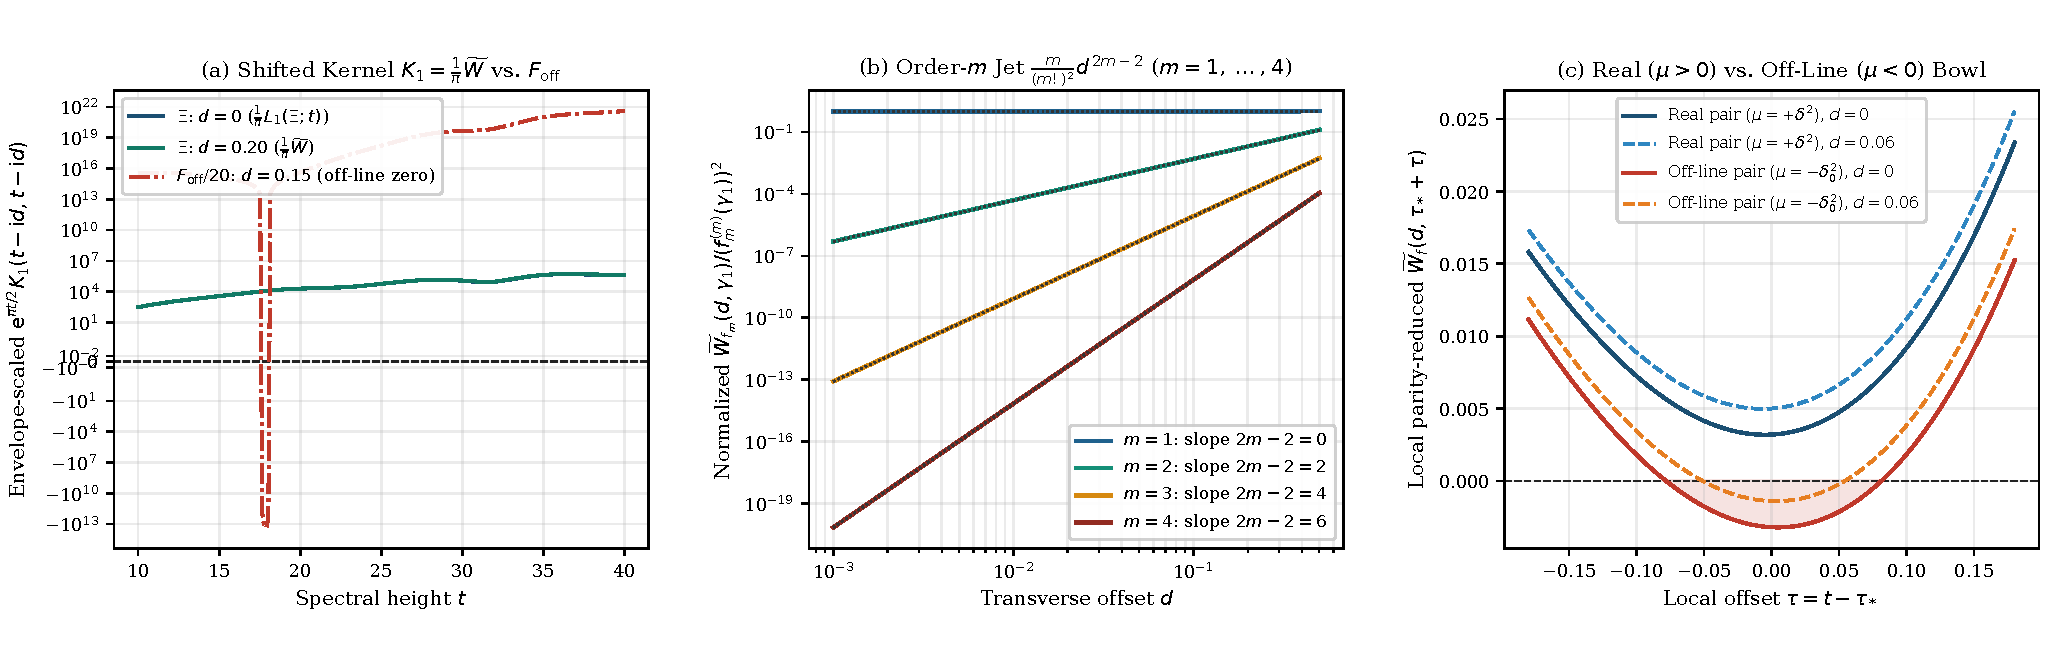
\includegraphics[width=\textwidth]{figures/fig1_debranges_kernel_and_lehmer_cascade.pdf}
  \caption{\textbf{(a)} Envelope-scaled diagonal kernel $\ee^{\pi t/2}K_1(t-\ii d, t-\ii d) = \frac{1}{\pi}\ee^{\pi t/2}\widetilde{W}(d,t)$ for $\Xi$ at $d = 0$ and $d = 0.20$ versus the off-critical zero perturbation $F_{\mathrm{off}}/20$ at $d = 0.15$, which dips strictly negative near $t = 17.85$ (Proposition~\ref{prop:hb_rh_equivalence}). \textbf{(b)} Log--log verification of the order-$m$ multiplicity jet $\widetilde{W}_{f_m}(d, \gamma_1)/(f_m^{(m)}(\gamma_1))^2 \sim \frac{m}{(m\fac)^2}d^{2m-2}$ for $m = 1,2,3,4$ (Theorem~\ref{thm:square_cascade}). \textbf{(c)} Unified local quadratic bowl (Theorem~\ref{thm:lehmer_bowl}): strictly positive for a real pair ($\mu = +\delta^2 > 0$) versus negative on $\tau^2 + d^2 < \delta_0^2$ for an off-critical conjugate pair ($\mu = -\delta_0^2 < 0$).}
  \label{fig:kernel_and_cascade}
\end{figure}

% ==============================================================================
% SECTION 4: LEIBNIZ-WRONSKIAN MULTIPLIERS, PRIME-POWER RECURSION & STIRLING
% ==============================================================================
\section{Leibniz--Wronskian Multipliers, Truncated Prime-Power Series, and Critical-Line Envelopes}\label{sec:leibniz_wronskian}

We next examine how $W(d,t)$ transforms under multiplication of $\Xi(z)$ by a holomorphic gauge factor $\mathcal{M}(z)$ and analyze the Dirichlet coefficients of truncated exponential Euler factors.

\begin{theorem}[Leibniz--Wronskian multiplier identity and local exclusion bounds]\label{thm:leibniz_wronskian}
Let $\mathcal{M}(z)$ be holomorphic on a domain $\Omega \subset \mathbb{C}$, and set $\Xi_{\mathcal{M}}(z) := \mathcal{M}(z)\Xi(z)$, $W_{\mathcal{M}}(d,t) := \frac{1}{2}\partial_d\lvert\Xi_{\mathcal{M}}(t-\ii d)\rvert^2$, and $W_{1,\mathcal{M}}(d,t) := \frac{1}{2}\partial_d\lvert\mathcal{M}(t-\ii d)\rvert^2$.
\begin{enumerate}[label=\textup{(\arabic*)},leftmargin=2.2em]
  \item \textbf{Unscaled and parity-reduced Leibniz--Wronskian laws:} For every $z = t - \ii d \in \Omega$,
  \begin{equation}\label{eq:W_M_unscaled}
    W_{\mathcal{M}}(d,t) = \lvert\mathcal{M}(t - \ii d)\rvert^2\,W(d,t) + \lvert\Xi(t - \ii d)\rvert^2\,W_{1,\mathcal{M}}(d,t).
  \end{equation}
  For $d \neq 0$, dividing by $d$ gives $\widetilde{W}_{\mathcal{M}}(d,t) = \lvert\mathcal{M}(z)\rvert^2\widetilde{W}(d,t) + \lvert\Xi(z)\rvert^2 d^{-1}W_{1,\mathcal{M}}(d,t)$. The quotient $\widetilde{W}_{1,\mathcal{M}}(d,t) := d^{-1}W_{1,\mathcal{M}}(d,t)$ extends continuously across $d = 0$ on $\Omega \cap \mathbb{R}$ if and only if $W_{1,\mathcal{M}}(0,t) \equiv 0$ (in particular, whenever $\mathcal{M}^\# = \mathcal{M}$), in which case
  \begin{equation}\label{eq:leibniz_wronskian_d0}
    L_1(\Xi_{\mathcal{M}}; t) = \bigl(\mathcal{M}(t)\bigr)^2 L_1(\Xi; t) + \bigl(\Xi(t)\bigr)^2 L_1(\mathcal{M}; t).
  \end{equation}
  \item \textbf{Point-wise zero-exclusion bounds:} If $z_0 = t_0 - \ii d_0 \in \Omega$ ($d_0 > 0$) satisfies $W_{\mathcal{M}}(d_0, t_0) > 0$, then $\Xi(z_0) \neq 0$ and $\mathcal{M}(z_0) \neq 0$, with explicit lower bounds
  \begin{align}
    \lvert\Xi(z_0)\rvert &\ge \mathcal{B}_{\mathrm{CS}}(d_0,t_0;\mathcal{M}) := \frac{W_{\mathcal{M}}(d_0,t_0)}{\lvert\mathcal{M}(z_0)\rvert\,\lvert\Xi_{\mathcal{M}}'(z_0)\rvert} > 0, \label{eq:B_CS_bound} \\
    \lvert\Xi(z_0)\rvert^2 + \lvert\Xi'(z_0)\rvert^2 &\ge \mathcal{B}_{\mathrm{dist}}(d_0,t_0;\mathcal{M}) := \frac{4\,W_{\mathcal{M}}(d_0,t_0)}{2\lvert W_{1,\mathcal{M}}(d_0,t_0)\rvert + \sqrt{\lvert\mathcal{M}(z_0)\rvert^4 + 4\,W_{1,\mathcal{M}}(d_0,t_0)^2}} > 0. \label{eq:B_dist_bound}
  \end{align}
  Conversely, any parasitic zero $\mathcal{M}(z_0) = 0$ forces $W_{1,\mathcal{M}}(d_0,t_0) = 0$ and $W_{\mathcal{M}}(d_0,t_0) = 0$.
\end{enumerate}
\end{theorem}

\begin{proof}
(1) Away from the isolated zeros of $\mathcal{M}$ and $\Xi$, $W(d,t) = \lvert\Xi(z)\rvert^2\Ima(\Xi'(z)/\Xi(z))$ and $\Xi_{\mathcal{M}}'/\Xi_{\mathcal{M}} = \Xi'/\Xi + \mathcal{M}'/\mathcal{M}$ yield \eqref{eq:W_M_unscaled}, which extends across isolated zeros by real-analyticity. Since $W_{1,\mathcal{M}}(d,t) = W_{1,\mathcal{M}}(0,t) + \widetilde{W}_{1,\mathcal{M}}(0,t)d + \mathcal{O}(d^2)$, $d^{-1}W_{1,\mathcal{M}}(d,t)$ has a finite limit as $d \to 0$ if and only if $W_{1,\mathcal{M}}(0,t) = \Ima(\overline{\mathcal{M}(t)}\mathcal{M}'(t)) = 0$; when $\mathcal{M}$ is real-valued on $\Omega\cap\mathbb{R}$, taking $d \to 0$ gives \eqref{eq:leibniz_wronskian_d0}.

(2) If $\Xi(z_0) = 0$ or $\mathcal{M}(z_0) = 0$, \eqref{eq:W_M_unscaled} gives $W_{\mathcal{M}}(d_0,t_0) = 0$. Cauchy--Schwarz on $W_{\mathcal{M}}(d_0,t_0) = \Ima(\overline{\mathcal{M}(z_0)\Xi(z_0)}\,\Xi_{\mathcal{M}}'(z_0))$ gives \eqref{eq:B_CS_bound}. Applying $\lvert W(d_0,t_0)\rvert \le \frac{1}{2}\eta\lvert\Xi(z_0)\rvert^2 + \frac{1}{2}\eta^{-1}\lvert\Xi'(z_0)\rvert^2$ ($\eta > 0$) to \eqref{eq:W_M_unscaled} and choosing $\eta > 0$ so that $\frac{1}{2}\lvert\mathcal{M}(z_0)\rvert^2\eta^{-1} = \frac{1}{2}\lvert\mathcal{M}(z_0)\rvert^2\eta + \lvert W_{1,\mathcal{M}}(d_0,t_0)\rvert$ solves a quadratic for the common coefficient, yielding \eqref{eq:B_dist_bound}.
\end{proof}

Next, we record the exact Fej\'er Bochner--Weil convolution formula and its strip residue jump when crossing $s = 1$ and any off-critical zeros.

\begin{proposition}[Fej\'er Bochner--Weil prime truncation and strip residues]\label{prop:bochner_weil}
For $X > 1$ and $U := \ln X > 0$, define the entire Fej\'er kernel $K_U(u) := \frac{1}{2\pi U}(\frac{\sin(Uu/2)}{u/2})^2$ ($\ge 0$ on $\mathbb{R}$), whose Fourier transform $\widehat{K}_U(\xi) = \int_{-\infty}^\infty K_U(u)\ee^{-\ii\xi u}\,\dd u = \max(0, 1 - \frac{\lvert\xi\rvert}{U})$ vanishes identically for $\lvert\xi\rvert \ge U$. Set $\mathcal{A}(d,\tau) := \Rea(\frac{1}{s} + \frac{1}{s-1} - \frac{1}{2}\ln\pi + \frac{1}{2}\psi(\frac{s}{2}))|_{s = \frac{1}{2}+d+\ii\tau}$.
\begin{enumerate}[label=\textup{(\arabic*)},leftmargin=2.2em]
  \item \textbf{Unconditional finite prime sum on $d > \frac{1}{2}$ ($\sigma > 1$):} For every $d > \frac{1}{2}$ and $t \in \mathbb{R}$,
  \begin{equation}\label{eq:bochner_weil_sigma_gt_1}
    \begin{aligned}
      \mathcal{L}_U(d,t) &:= \int_{-\infty}^{\infty} K_U(u)\,\frac{W(d,t+u)}{\lvert\Xi(t+u-\ii d)\rvert^2}\,\dd u \\
      &= \int_{-\infty}^{\infty} K_U(u)\,\mathcal{A}(d,t+u)\,\dd u
         - \sum_{2 \le n < X}\frac{\Lambda(n)}{n^{1/2+d}}\left(1 - \frac{\ln n}{U}\right)\cos(t\ln n).
    \end{aligned}
  \end{equation}
  \item \textbf{Pole and zero-residue terms inside $0 < d < \frac{1}{2}$ ($\frac{1}{2} < \sigma < 1$):} For $0 < d < \frac{1}{2}$ such that $\zeta(\frac{1}{2}+d+\ii\tau) \neq 0$ for all $\tau \in \mathbb{R}$, $\mathcal{L}_U(d,t)$ equals the right-hand side of \eqref{eq:bochner_weil_sigma_gt_1} \emph{plus} the $s = 1$ pole contribution and off-critical zero sum
  \begin{equation}\label{eq:bochner_weil_strip_residues}
    +2\pi\Rea K_U\!\Bigl(t + \ii\bigl(\tfrac{1}{2}-d\bigr)\Bigr)
    - 2\pi\sum_{d_\rho > d} m_\rho\,\Rea K_U\!\bigl((t - \gamma_\rho) + \ii(d_\rho - d)\bigr),
  \end{equation}
  where $\rho = \frac{1}{2} + d_\rho + \ii\gamma_\rho$ ranges over any distinct non-trivial zeros of $\zeta(s)$ with $d_\rho > d$ of multiplicity $m_\rho \ge 1$.
\end{enumerate}
\end{proposition}

\begin{proof}
Since $\frac{W(d,\tau)}{\lvert\Xi(\tau-\ii d)\rvert^2} = \Rea\frac{\xi'(\frac{1}{2}+d+\ii\tau)}{\xi(\frac{1}{2}+d+\ii\tau)} = \mathcal{A}(d,\tau) + \Rea\frac{\zeta'(\frac{1}{2}+d+\ii\tau)}{\zeta(\frac{1}{2}+d+\ii\tau)}$, for $d > \frac{1}{2}$ the Dirichlet series $-\frac{\zeta'(s)}{\zeta(s)} = \sum_{n=2}^\infty \Lambda(n)n^{-s}$ converges absolutely and uniformly in $\tau$. Because $K_U \in L^1(\mathbb{R})$ is even and $\mathcal{A}(d,t+u)K_U(u) = \mathcal{O}(\lvert u\rvert^{-2}\ln\lvert u\rvert)$ as $\lvert u\rvert \to \infty$, Fubini's theorem integrates $-\Lambda(n)n^{-1/2-d}\cos((t+u)\ln n)$ term-by-term to $-\Lambda(n)n^{-1/2-d}\widehat{K}_U(\ln n)\cos(t\ln n)$, which vanishes for $n \ge \ee^U = X$, proving \eqref{eq:bochner_weil_sigma_gt_1}. For $0 < d < \frac{1}{2}$, $K_U(w)$ is entire and $\mathcal{O}(\lvert\Rea w\rvert^{-2})$ uniformly on horizontal strips, while $\zeta'(s)/\zeta(s) = \mathcal{O}(\ln^2(\lvert\Ima s\rvert+2))$ along horizontal zero-free contours \cite[Section~9.6]{Titchmarsh1986}; shifting $\Rea(s) = \frac{1}{2}+d$ rightward to $\sigma_1 > 1$ crosses the simple pole at $s = 1$ (residue $-1$) and each zero $\rho$ with $d_\rho > d$ (residue $+m_\rho$), yielding \eqref{eq:bochner_weil_strip_residues} upon taking real parts.
\end{proof}

We now establish the combinatorial coefficient bounds for truncated exponential Euler factors on $\Rea(s) > 1$ (compare the truncated Euler-product constructions of Gonek, Hughes, and Keating \cite{GonekHughesKeating2007}).

\begin{theorem}[Bounded residual coefficients of truncated exponential Euler factors]\label{thm:prime_gauge_sieve}
For any cutoff $X \ge 2$, define the entire zero-free exponential prime-power factor
\begin{equation}\label{eq:E_X_def}
  E_X(s) := \exp\!\left(-\sum_{2 \le k \le X}\frac{\Lambda(k)}{\ln k}\,k^{-s}\right),
\end{equation}
and for $\Rea(s) > 1$ expand the residual Dirichlet series $\zeta_X(s) := E_X(s)\zeta(s) = \exp(\sum_{k > X}\frac{\Lambda(k)}{\ln k}k^{-s}) = 1 + \sum_{n > X} b_n^{\mathcal{E}}(X)\,n^{-s}$.
\begin{enumerate}[label=\textup{(\arabic*)},leftmargin=2.2em]
  \item \textbf{Unit-interval coefficient bounds and quadratic prime-power window:} The coefficients $b_n^{\mathcal{E}}(X)$ satisfy the recursion $b_1^{\mathcal{E}}(X) = 1$ and
  \begin{equation}\label{eq:b_n_E_recursion}
    b_n^{\mathcal{E}}(X)\ln n = \sum_{\substack{k \mid n \\ k > X}} b_{n/k}^{\mathcal{E}}(X)\,\Lambda(k) \qquad (n \ge 2),
  \end{equation}
  together with the exact bounds
  \begin{equation}\label{eq:b_n_E_bounds}
    b_n^{\mathcal{E}}(X) = 0 \;\; (2 \le n \le X), \quad
    0 \le b_n^{\mathcal{E}}(X) \le 1 \;\; (n \ge 1), \quad
    b_n^{\mathcal{E}}(X) = \frac{\Lambda(n)}{\ln n} \;\; \bigl(X < n < (\lfloor X\rfloor + 1)^2\bigr).
  \end{equation}
  \item \textbf{Residual theta-tail monotonicity:} For $\psi_X(x) := \sum_{n=2}^\infty b_n^{\mathcal{E}}(X)\ee^{-\pi n^2 x}$ ($x > 0$) and every integer $r \ge 0$,
  \begin{equation}\label{eq:theta_tail_bound}
    0 \le (-1)^r \psi_X^{(r)}(x) \le \sum_{n = \lfloor X\rfloor + 1}^{\infty} (\pi n^2)^r \ee^{-\pi n^2 x}.
  \end{equation}
\end{enumerate}
\end{theorem}

\begin{proof}
See Appendix~\ref{app:overshoot_proof}.
\end{proof}

Finally, to relate $c_1(t) = L_1(\Xi; t)$ on the critical line $d = 0$ accurately to Hardy's function $Z(t) := \ee^{\ii\vartheta(t)}\zeta(\frac{1}{2}+\ii t)$ (where $\vartheta(t) := \Ima\ln\Gamma(\frac{1}{4}+\ii\frac{t}{2}) - \frac{t}{2}\ln\pi$), we record the exact Stirling envelope factorization.

\begin{proposition}[Exact critical-line envelope identity between $\Xi(t)$ and $Z(t)$]\label{prop:stirling_bridge}
For all $t \in \mathbb{R}$, $\Xi(t) = -E_0(t)\,Z(t)$, where the positive even real-analytic envelope
\begin{equation}\label{eq:E0_def}
  E_0(t) := \frac{1}{2}\left(t^2 + \frac{1}{4}\right)\pi^{-1/4}\left\lvert\Gamma\!\left(\frac{1}{4} + \ii\frac{t}{2}\right)\right\rvert
  = \frac{t^2}{\sqrt{2}}\left(\frac{2\pi}{t}\right)^{1/4}\ee^{-\pi t/4}\Bigl(1 + \mathcal{O}(t^{-1})\Bigr) \qquad (t \to +\infty)
\end{equation}
satisfies the exact Laguerre decomposition
\begin{equation}\label{eq:c1_Z_bridge}
  c_1(t) = L_1(\Xi; t) = E_0(t)^2\,L_1(Z; t) + Z(t)^2\,L_1(E_0; t),
\end{equation}
with $L_1(E_0; t) > 0$ for all $\lvert t\rvert \ge 1$.
\end{proposition}

\begin{proof}
Since $(\frac{1}{2}+\ii t)(-\frac{1}{2}+\ii t) = -(t^2 + \frac{1}{4})$ and $\Gamma(\frac{1}{4}+\ii\frac{t}{2})\pi^{-\ii t/2} = \lvert\Gamma(\frac{1}{4}+\ii\frac{t}{2})\rvert\ee^{\ii\vartheta(t)}$, the definition of $\xi(\frac{1}{2}+\ii t)$ gives $\Xi(t) = -E_0(t)Z(t)$, and Stirling's formula $\lvert\Gamma(\frac{1}{4}+\ii\frac{t}{2})\rvert = \sqrt{2\pi}(t/2)^{-1/4}\ee^{-\pi t/4}(1 + \mathcal{O}(t^{-1}))$ gives the asymptotic in \eqref{eq:E0_def} (note the polynomial factor $t^2$ and minus sign separating $\Xi(t)$ from $\ee^{-\pi t/4}t^{-1/4}Z(t)$). Applying \eqref{eq:leibniz_wronskian_d0} to $\Xi(t) = (-E_0(t))Z(t)$ gives \eqref{eq:c1_Z_bridge}. Differentiating $\ln E_0(t) = -\ln 2 + \ln(t^2+\frac{1}{4}) - \frac{1}{4}\ln\pi + \Rea\ln\Gamma(\frac{1}{4}+\ii\frac{t}{2})$ twice yields
\begin{equation*}
  -\frac{\dd^2}{\dd t^2}\ln E_0(t) = \frac{2(t^2 - \frac{1}{4})}{(t^2 + \frac{1}{4})^2} + \frac{1}{4}\Rea\psi'\!\left(\frac{1}{4} + \ii\frac{t}{2}\right).
\end{equation*}
For $\lvert t\rvert \ge 1$, the first term is $\ge \frac{2(3/4)}{(5/4)^2} = \frac{24}{25} = 0.96$, while by Binet's formula $\lvert\psi'(w) - w^{-1} - \frac{1}{2}w^{-2}\rvert \le \frac{1}{6}\lvert w\rvert^{-3}$ on $\Rea(w) = \frac{1}{4}$, $\frac{1}{4}\lvert\Rea\psi'(\frac{1}{4}+\ii\frac{t}{2})\rvert < 0.70$, so $L_1(E_0; t) = -E_0(t)^2\frac{\dd^2}{\dd t^2}\ln E_0(t) > 0$ for all $\lvert t\rvert \ge 1$.
\end{proof}

\begin{figure}[htbp]
  \centering
  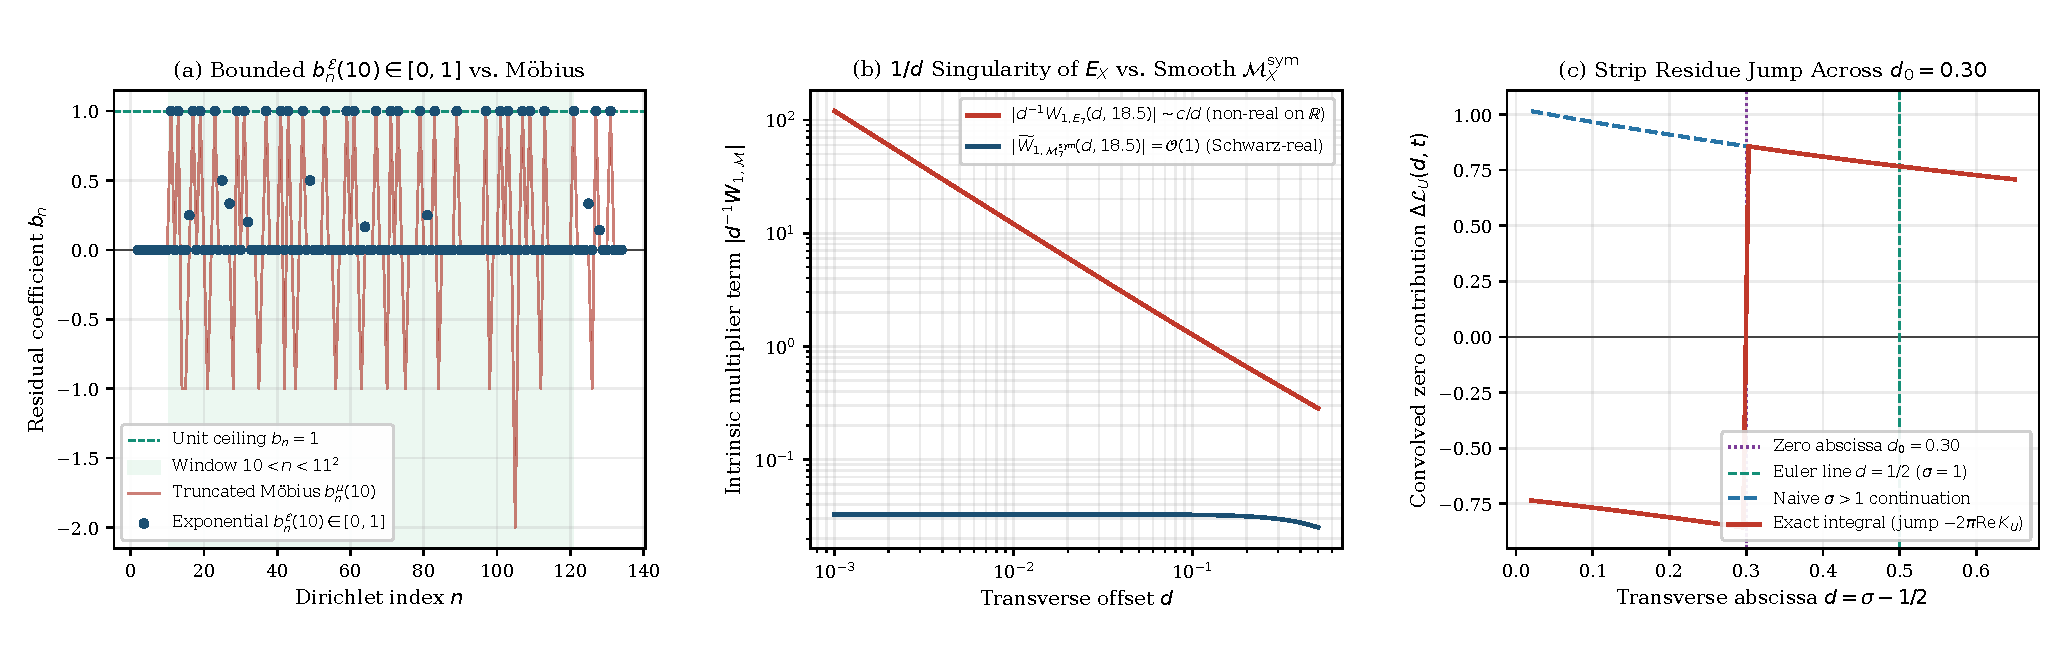
\includegraphics[width=\textwidth]{figures/fig2_leibniz_wronskian_and_gabcke_closure.pdf}
  \caption{\textbf{(a)} Residual Dirichlet coefficients $b_n^{\mathcal{E}}(10) \in [0,1]$ of $\zeta_{10}(s) = E_{10}(s)\zeta(s)$ showing prime-power purity on $10 < n < 11^2 = 121$ versus the $>1$ overshoot of truncated M\"obius convolution (Theorem~\ref{thm:prime_gauge_sieve}). \textbf{(b)} Log--log transverse scan at $t = 18.5$: unsymmetrized $\lvert d^{-1}W_{1,E_7}(d,18.5)\rvert \sim c/d$ diverges as $d \to 0^+$ due to broken Schwarz reflection on $\mathbb{R}$, whereas conjugate-symmetrized $\lvert\widetilde{W}_{1,\mathcal{M}_7^{\mathrm{sym}}}(d,18.5)\rvert$ remains bounded (Section~\ref{sec:obstructions}). \textbf{(c)} Fej\'er Bochner--Weil contour shift across an off-critical zero at $d_0 = 0.30$: exact match for $d > d_0$ versus the residue jump $-2\pi\Rea K_U((t-\gamma_0)+\ii(d_0-d))$ on $0 < d < d_0$ (Proposition~\ref{prop:bochner_weil}).}
  \label{fig:leibniz_and_obstructions}
\end{figure}

% ==============================================================================
% SECTION 5: NUMERICAL AND INTERVAL VERIFICATION
% ==============================================================================
\section{High-Precision Numerical and Interval Verification}\label{sec:numerical}

All analytical identities, counterexamples, and corrected critical-line constants in Sections~\ref{sec:debranges}--\ref{sec:leibniz_wronskian} are verified in the standalone script \nolinkurl{scripts/verify_paper4_debranges_lehmer_cascade.py} using $50$-digit \texttt{mpmath}, $55$-digit directed-rounding interval arithmetic (\texttt{mpmath.iv}), and $560$-digit local Taylor evaluation.

\begin{enumerate}[label=\textup{(\arabic*)},leftmargin=2.2em]
  \item \textbf{Canonical Wigner and Cauchy--Pick audit (Table~\ref{tab:debranges_audit}):} Across representative strip points, the canonical Wigner integral \eqref{eq:W_Wigner_canonical} matches $\frac{1}{2}\partial_d\lvert\Xi(t-\ii d)\rvert^2$ to relative error $\le 1.05 \times 10^{-57}$ at $65$-digit working precision. For $\alpha \in \{0.25, 1.0, 2.5\}$, the diagonal identity \eqref{eq:debranges_boxed}, Schur defect \eqref{eq:schur_defect}, and $5\times 5$ divided-difference matrix \eqref{eq:gram_divided_diff} hold to $\le 1.80 \times 10^{-50}$. Using $N_u = 160$ composite trapezoidal intervals on $u \in [0, 1.55]$ in \texttt{mpmath.iv}---where analyticity of $\Phi(u)$ on $\lvert\Ima(u)\rvert \le 0.35 < \frac{\pi}{8}$ yields a proven Trefethen--Weideman discretization error $< 10^{-65}$ for $d \le 0.50, t \le 42$ (Paper~II \cite[Lemma~A.1(c)]{Missiaen2026Paper2})---we obtain rigorous enclosures of $\ee^{\pi t/2}K_1(t-\ii d, t-\ii d) > 0$ of width $\le 2.01 \times 10^{-39}$. Note that finite-box verification at low height is purely illustrative, since RH is already rigorously established up to $t \le 3 \times 10^{12}$ by Gram \cite{Gram1903}, Titchmarsh \cite{TitchmarshComrie1936}, and Platt and Trudgian \cite{PlattTrudgian2021}.
  \item \textbf{True critical-line extrema $\tau_1, \tau_2$ and $550$-digit coalescence jet (Table~\ref{tab:coalescence_550}):} Because $\Xi(t) = -E_0(t)Z(t)$ contains the exponential factor $\ee^{-\pi t/4}$, the roots of $\Xi'(t) = 0$ are shifted substantially downward relative to the extrema of Hardy's $Z$-function: on $(\gamma_1, \gamma_2)$ and $(\gamma_2, \gamma_3)$, bracketed root-finding gives
  \begin{equation}\label{eq:true_tau1_tau2}
    \tau_1 = 15.585708589829342345\dots, \qquad
    \tau_2 = 22.097977280400902098\dots,
  \end{equation}
  whereas the first positive root of $Z'(t) = 0$ lies at $t_{Z',1} = 17.882582076936682719\dots$ (and the zeroth Gram point $\vartheta(g_0) = 0$ at $g_0 = 17.8455995405\dots$). Anchoring the local deformation $f_\delta(z) := \Xi(z) - \Xi(\tau_1) - \frac{1}{2}\Xi''(\tau_1)\delta^2$ at the true extremum $\tau_1$ at $560$-digit precision confirms that as $\Delta\gamma = 2\delta + \mathcal{O}(\delta^3)$ shrinks from $10^{-1}$ to $10^{-250}$, $c_1(f_\delta; \tau_1) = \frac{1}{2}(\Xi''(\tau_1))^2\delta^2 \to 0^+$ quadratically while $c_3(f_\delta; \tau_1)$ converges to $\frac{1}{2}(\Xi''(\tau_1))^2 = 1.00779672376\dots \times 10^{-7} > 0$. Evaluating Lehmer's historical pair $(\gamma_{6709}, \gamma_{6710})$ ($\Delta\gamma \approx 0.03769850$, $\tau_* \approx 7005.08171569$) similarly confirms $\mu = +3.55140363 \times 10^{-4} > 0$, $\ee^{\pi\tau_*/2}c_1(\tau_*) \approx +3.1959 \times 10^{12} > 0$, and $\ee^{\pi\tau_*/2}c_3(\tau_*) \approx +9.0067 \times 10^{15} > 0$.
\end{enumerate}

\begin{table}[htbp]
  \centering
  \caption{Verification of the diagonal kernel identity $K_1(z,z) = \frac{1}{\pi}\widetilde{W}(d,t)$ (Theorem~\ref{thm:debranges_kernel}) via $55$-digit \texttt{mpmath.iv} enclosures ($N_u = 160$, proven strip error $< 10^{-65}$), contrasted with the off-critical zero perturbation $F_{\mathrm{off}}(z)$ at $z = 17.85 - 0.15\ii$.}
  \label{tab:debranges_audit}
  \renewcommand{\arraystretch}{1.15}
  \begin{tabular}{@{}llrrr@{}}
    \toprule
    Function & Point $(d, t)$ & $\ee^{\pi t/2} K_1(z,z)$ & Interval Width & $\lvert\Theta_1(z)\rvert$ \\
    \midrule
    $\Xi(z)$ & $(0.05,\; 14.13472514)$ & $+2.67305185 \times 10^{3}$ & $1.16 \times 10^{-48}$ & $0.985410 < 1$ \\
    $\Xi(z)$ & $(0.20,\; 15.58570859)$ & $+4.94383597 \times 10^{3}$ & $2.06 \times 10^{-48}$ & $0.761529 < 1$ \\
    $\Xi(z)$ & $(0.35,\; 21.02203964)$ & $+2.27454159 \times 10^{4}$ & $7.53 \times 10^{-46}$ & $0.684912 < 1$ \\
    $\Xi(z)$ & $(0.50,\; 25.01085758)$ & $+6.37572008 \times 10^{4}$ & $2.37 \times 10^{-44}$ & $0.619404 < 1$ \\
    $\Xi(z)$ & $(0.25,\; 37.58617816)$ & $+5.02658084 \times 10^{5}$ & $2.01 \times 10^{-39}$ & $0.793118 < 1$ \\
    \midrule
    $F_{\mathrm{off}}(z)$ & $(0.15,\; 17.85000000)$ & $-4.48208012 \times 10^{14}$ & --- & $1.306865 > 1$ \\
    \bottomrule
  \end{tabular}
\end{table}

\begin{table}[htbp]
  \centering
  \caption{$550$-digit local coalescence audit for $f_\delta(z) = \Xi(z) - \Xi(\tau_1) - \frac{1}{2}\Xi''(\tau_1)\delta^2$ anchored at the true first positive root $\tau_1 = 15.5857085898293423\dots$ of $\Xi'(t)=0$, with double-zero floor $c_{3,\mathrm{floor}} := \frac{1}{2}(\Xi''(\tau_1))^2 = 1.00779672376 \times 10^{-7}$.}
  \label{tab:coalescence_550}
  \renewcommand{\arraystretch}{1.15}
  \begin{tabular}{@{}lllll@{}}
    \toprule
    Target $2\delta$ & True Zero Gap $\Delta\gamma$ & $c_1(f_\delta; \tau_1)$ & $c_3(f_\delta; \tau_1)$ & $\lvert c_3 - c_{3,\mathrm{floor}}\rvert / c_{3,\mathrm{floor}}$ \\
    \midrule
    $10^{-1}$   & $1.0001473951 \times 10^{-1}$ & $2.51949181 \times 10^{-10}$  & $1.00748153 \times 10^{-7}$ & $3.12759 \times 10^{-4}$ \\
    $10^{-3}$   & $1.0000000147 \times 10^{-3}$ & $2.51949181 \times 10^{-14}$  & $1.00779669 \times 10^{-7}$ & $3.12759 \times 10^{-8}$ \\
    $10^{-6}$   & $1.0000000000 \times 10^{-6}$ & $2.51949181 \times 10^{-20}$  & $1.00779672 \times 10^{-7}$ & $3.12759 \times 10^{-14}$ \\
    $10^{-12}$  & $1.0000000000 \times 10^{-12}$ & $2.51949181 \times 10^{-32}$ & $1.00779672 \times 10^{-7}$ & $3.12759 \times 10^{-26}$ \\
    $10^{-30}$  & $1.0000000000 \times 10^{-30}$ & $2.51949181 \times 10^{-68}$ & $1.00779672 \times 10^{-7}$ & $3.12759 \times 10^{-62}$ \\
    $10^{-100}$ & $1.0000000000 \times 10^{-100}$ & $2.51949181 \times 10^{-208}$ & $1.00779672 \times 10^{-7}$ & $3.12759 \times 10^{-202}$ \\
    $10^{-250}$ & $1.0000000000 \times 10^{-250}$ & $2.51949181 \times 10^{-508}$ & $1.00779672 \times 10^{-7}$ & $3.12759 \times 10^{-502}$ \\
    \bottomrule
  \end{tabular}
\end{table}

% ==============================================================================
% SECTION 6: SCOPE, LIMITATIONS, AND EXPLICIT OBSTRUCTIONS
% ==============================================================================
\section{Scope, Limitations, and Explicit Obstructions}\label{sec:obstructions}

We summarize the structural obstructions explaining why the identities in Sections~\ref{sec:debranges}--\ref{sec:leibniz_wronskian} do not yield an unconditional proof of off-critical zero-freeness:
\begin{enumerate}[label=\textup{(\arabic*)},leftmargin=2.2em]
  \item \textbf{Hermite--Biehler circularity (Proposition~\ref{prop:hb_rh_equivalence}):} Because $K_\alpha(t-\ii d, t-\ii d) = \frac{\alpha}{\pi}\widetilde{W}(d,t)$ is an exact scalar multiple of $\widetilde{W}(d,t)$, invoking de Branges' reproducing-kernel Hilbert space $\mathcal{H}(E_\alpha^\#)$ requires knowing $E_\alpha^\# \in \mathcal{HB}(\mathbb{C}_+)$ beforehand, which is equivalent to RH \cite{Levinson1974,Lagarias2005,Lagarias2006}.
  \item \textbf{Davenport--Heilbronn sign reversal in the quadratic bowl (Theorem~\ref{thm:lehmer_bowl}):} The order-$m$ cascade \eqref{eq:cascade_pure_square} and positive bowl $\frac{1}{2}(f''(\tau_*))^2(\delta^2 + \tau^2 + d^2)$ hold conditionally on the zeros being \emph{real} ($\mu \ge 0$). Any real-entire function possessing off-critical conjugate zeros near $\mathbb{R}$---such as the Davenport--Heilbronn function \cite{DavenportHeilbronn1936,Titchmarsh1986}---exhibits critical-line extrema with $\mu = -\delta_0^2 < 0$ ($L_1 < 0$), reversing the bowl floor to $-\frac{1}{2}(f''(\tau_*))^2\delta_0^2 < 0$.
  \item \textbf{Broken Schwarz reflection of $E_X$ versus broken symmetry of $\mathcal{M}_X^{\mathrm{sym}}$:} Set $\mathcal{M}_X(z) := E_X(\frac{1}{2}+\ii z)$ with $E_X$ from \eqref{eq:E_X_def}. Since $\mathcal{M}_X'(z)/\mathcal{M}_X(z) = \ii\sum_{2\le n\le X}\Lambda(n)n^{-1/2-\ii z}$, on the critical line $d = 0$ one has
  \begin{equation}\label{eq:W_1E_d0_nonzero}
    W_{1,\mathcal{M}_X}(0,t) = \bigl\lvert E_X(\tfrac{1}{2}+\ii t)\bigr\rvert^2 \sum_{2 \le n \le X}\frac{\Lambda(n)}{\sqrt{n}}\cos(t\ln n) \not\equiv 0,
  \end{equation}
  so $d^{-1}W_{1,\mathcal{M}_X}(d,t)$ diverges like $d^{-1}W_{1,\mathcal{M}_X}(0,t)$ as $d \to 0^+$ (Figure~\ref{fig:leibniz_and_obstructions}(b)). Symmetrizing via $\mathcal{M}_X^{\mathrm{sym}}(z) := E_X(\frac{1}{2}+\ii z)E_X(\frac{1}{2}-\ii z) = \exp(-2\sum_{2\le n\le X}\frac{\Lambda(n)}{n^{1/2}\ln n}\cos(z\ln n))$ restores $\mathcal{M}^\# = \mathcal{M}$ and yields the smooth parity-reduced Wronskian
  \begin{equation}\label{eq:W_1Msym_explicit}
    \widetilde{W}_{1,\mathcal{M}_X^{\mathrm{sym}}}(d,t)
    = -2\bigl\lvert\mathcal{M}_X^{\mathrm{sym}}(t-\ii d)\bigr\rvert^2 \sum_{2 \le n \le X}\frac{\Lambda(n)\ln n}{\sqrt{n}}\,\sinch(d\ln n)\cos(t\ln n).
  \end{equation}
  However, two simultaneous obstructions arise: first, $E_X(s) \neq E_X(1-s)$ breaks the functional equation of $\xi(s)$, so neither $E_X(s)\xi(s)$ nor $\mathcal{M}_X^{\mathrm{sym}}(z)\Xi(z)$ admits a symmetric Riemann--Siegel main sum with coefficients $b_n^{\mathcal{E}}(X)$; second, by Kronecker's linear independence of $\{\ln p\}$, \eqref{eq:W_1Msym_explicit} has mean zero in $t$ and oscillates between positive and negative values, subtracting from $\lvert\mathcal{M}_X^{\mathrm{sym}}\rvert^2\widetilde{W}(d,t)$ in \eqref{eq:W_M_unscaled} whenever primes align in phase.
  \item \textbf{Strip residue barrier and Gabcke domain limits:} In Proposition~\ref{prop:bochner_weil}, the prime-truncated identity \eqref{eq:bochner_weil_sigma_gt_1} holds unconditionally only on $d > \frac{1}{2}$ ($\sigma > 1$, cf.\ Hinkkanen \cite{Hinkkanen1997}); inside $0 < d < \frac{1}{2}$, omitting the zero-residue sum in \eqref{eq:bochner_weil_strip_residues} assumes a priori that no zeros lie to the right of $\frac{1}{2}+d$, while Voronin's universality theorem \cite{Voronin1975} governs the arbitrary phase behavior of $\zeta'(s)/\zeta(s)$ on $(\frac{1}{2}, 1)$. Likewise, Gabcke's explicit Riemann--Siegel remainder bounds \cite{Gabcke1979} apply strictly to unmodified $Z(t)$ ($b_n \equiv 1$, $d = 0$, $t \ge 200$) and cannot be extrapolated off the critical line ($d > 0$) or to sieved weights $b_n^{\mathcal{E}}(X)$; even on $d = 0$, extreme Skewes-type phase alignments allow the main-sum approximation of $L_1(Z; t)$ to dip below remainder thresholds near close zero pairs, requiring Turing zero-counting \cite{Turing1953,PlattTrudgian2021} rather than main-sum dominance alone.
\end{enumerate}

% ==============================================================================
% APPENDICES
% ==============================================================================
\appendix

\section{Derivation of the Cauchy--Pick Divided-Difference Matrix}\label{app:cauchy_pick}

\begin{proof}[Proof of Proposition~\ref{prop:cauchy_pick_gram}]
Let $z_j, z_k \in \mathbb{C}_-$. Expanding $E_\alpha(z_j)\overline{E_\alpha(z_k)}$ and $E_\alpha^\#(z_j)\overline{E_\alpha^\#(z_k)}$ from \eqref{eq:E_alpha_def} gives
\begin{align*}
  E_\alpha(z_j)\overline{E_\alpha(z_k)}
  &= \Xi(z_j)\overline{\Xi(z_k)} + \alpha^2\Xi'(z_j)\overline{\Xi'(z_k)}
     + \ii\alpha\Bigl(\Xi(z_j)\overline{\Xi'(z_k)} - \Xi'(z_j)\overline{\Xi(z_k)}\Bigr), \\
  E_\alpha^\#(z_j)\overline{E_\alpha^\#(z_k)}
  &= \Xi(z_j)\overline{\Xi(z_k)} + \alpha^2\Xi'(z_j)\overline{\Xi'(z_k)}
     - \ii\alpha\Bigl(\Xi(z_j)\overline{\Xi'(z_k)} - \Xi'(z_j)\overline{\Xi(z_k)}\Bigr).
\end{align*}
Subtracting the second line from the first cancels the zeroth-order and $\alpha^2$ products for all pairs $(j,k)$, leaving $2\ii\alpha(\Xi(z_j)\overline{\Xi'(z_k)} - \Xi'(z_j)\overline{\Xi(z_k)})$. Dividing by $2\pi\ii(z_j - \bar{z}_k) \neq 0$ yields \eqref{eq:gram_divided_diff}.
\end{proof}

\section{Proof of the Truncated Exponential Euler Coefficient Bounds}\label{app:overshoot_proof}

\begin{proof}[Proof of Theorem~\ref{thm:prime_gauge_sieve}]
(1) For $\Rea(s) > 1$, $\ln\zeta_X(s) = \sum_{k > X}\frac{\Lambda(k)}{\ln k}k^{-s}$ converges absolutely. Differentiating $\zeta_X(s) = \sum_{n=1}^\infty b_n^{\mathcal{E}}(X)n^{-s}$ gives $-\zeta_X'(s) = \zeta_X(s)(-\ln\zeta_X(s))'$, i.e.,
\begin{equation*}
  \sum_{n=2}^{\infty} b_n^{\mathcal{E}}(X)(\ln n)\,n^{-s}
  = \left(\sum_{m=1}^{\infty} b_m^{\mathcal{E}}(X)\,m^{-s}\right)\left(\sum_{k > X}\Lambda(k)\,k^{-s}\right).
\end{equation*}
Equating coefficients of $n^{-s}$ yields \eqref{eq:b_n_E_recursion} with $b_1^{\mathcal{E}}(X) = 1$. For $2 \le n \le X$, the divisor set $\{k \mid n : k > X\}$ is empty, so $b_n^{\mathcal{E}}(X) = 0$. Since $\Lambda(k) \ge 0$, strong induction on \eqref{eq:b_n_E_recursion} gives $b_n^{\mathcal{E}}(X) \ge 0$ for all $n \ge 1$. Assuming $b_m^{\mathcal{E}}(X) \le 1$ for all $1 \le m < n$, \eqref{eq:b_n_E_recursion} and the fundamental divisor identity $\sum_{k \mid n}\Lambda(k) = \ln n$ give
\begin{equation*}
  b_n^{\mathcal{E}}(X)\ln n = \sum_{\substack{k \mid n \\ k > X}} b_{n/k}^{\mathcal{E}}(X)\,\Lambda(k)
  \le \sum_{\substack{k \mid n \\ k > X}}\Lambda(k) \le \sum_{k \mid n}\Lambda(k) = \ln n,
\end{equation*}
proving $b_n^{\mathcal{E}}(X) \le 1$ for all $n \ge 1$. Finally, let $X < n < (\lfloor X\rfloor + 1)^2$. For any $k \mid n$ with $k > X$, we have $k \ge \lfloor X\rfloor + 1$, so $n/k < \lfloor X\rfloor + 1$, whence $1 \le n/k \le \lfloor X\rfloor \le X$. Because $b_m^{\mathcal{E}}(X) = 0$ for $2 \le m \le X$, only $n/k = 1$ ($k = n$) contributes to \eqref{eq:b_n_E_recursion}, giving $b_n^{\mathcal{E}}(X)\ln n = b_1^{\mathcal{E}}(X)\Lambda(n) = \Lambda(n)$.

(2) Differentiating $\psi_X(x)$ $r$ times term-by-term for $x > 0$ gives
\begin{equation*}
  (-1)^r\psi_X^{(r)}(x) = \sum_{n=\lfloor X\rfloor+1}^{\infty} b_n^{\mathcal{E}}(X)(\pi n^2)^r\ee^{-\pi n^2 x},
\end{equation*}
and applying $0 \le b_n^{\mathcal{E}}(X) \le 1$ yields \eqref{eq:theta_tail_bound}.
\end{proof}

\section*{Use of AI and Computational Tools}

\textbf{Gemini} (Google DeepMind) was used interactively to assist with symbolic verification of the divided-difference and Taylor jet identities, literature cross-checks, \LaTeX{} manuscript preparation, and implementation of the Python/\texttt{mpmath}/\texttt{mpmath.iv} verification script (\nolinkurl{scripts/verify_paper4_debranges_lehmer_cascade.py}). All mathematical proofs, domain conditions, counterexamples, citations, and numerical outputs were independently checked and verified.

\begin{thebibliography}{99}

\bibitem{ConreyLi2000}
J.~B.~Conrey and X.-J.~Li,
\emph{A note on some positivity conditions related to zeta and $L$-functions},
Internat.\ Math.\ Res.\ Notices \textbf{2000} (2000), no.~18, 929--940.

\bibitem{CsordasNorfolkVarga1986}
G.~Csordas, T.~S.~Norfolk, and R.~S.~Varga,
\emph{The Riemann hypothesis and the Tur\'an inequalities},
Trans.\ Amer.\ Math.\ Soc.\ \textbf{296} (1986), no.~2, 521--541.

\bibitem{CsordasSmithVarga1994}
G.~Csordas, W.~Smith, and R.~S.~Varga,
\emph{Lehmer pairs of zeros, the de Bruijn--Newman constant $\Lambda$, and the Riemann hypothesis},
Constr.\ Approx.\ \textbf{10} (1994), no.~1, 107--129.

\bibitem{CsordasVarga1990}
G.~Csordas and R.~S.~Varga,
\emph{Necessary and sufficient conditions and the Riemann hypothesis},
Adv.\ Appl.\ Math.\ \textbf{11} (1990), no.~3, 328--357.

\bibitem{DavenportHeilbronn1936}
H.~Davenport and H.~Heilbronn,
\emph{On the zeros of certain Dirichlet series.~I, II},
J.\ London Math.\ Soc.\ \textbf{11} (1936), 181--185, 307--312.

\bibitem{deBranges1968}
L.~de~Branges,
\emph{Hilbert Spaces of Entire Functions},
Prentice-Hall, Englewood Cliffs, NJ, 1968.

\bibitem{deBranges1986}
L.~de~Branges,
\emph{The Riemann hypothesis for Hilbert spaces of entire functions},
Bull.\ Amer.\ Math.\ Soc.\ (N.S.) \textbf{15} (1986), no.~1, 1--17.

\bibitem{Gabcke1979}
W.~Gabcke,
\emph{Neue Herleitung und explizite Restabsch\"atzung der Riemann-Siegel-Formel},
Ph.D.\ Dissertation, Georg-August-Universit\"at G\"ottingen, 1979.

\bibitem{GonekHughesKeating2007}
S.~M.~Gonek, C.~P.~Hughes, and J.~P.~Keating,
\emph{Multiplicative chaos and the Riemann zeta function},
Duke Math.\ J.\ \textbf{136} (2007), no.~3, 507--536.

\bibitem{Gram1903}
J.-P.~Gram,
\emph{Note sur les z\'eros de la fonction $\zeta(s)$ de Riemann},
Acta Math.\ \textbf{27} (1903), 289--304.

\bibitem{Hinkkanen1997}
A.~Hinkkanen,
\emph{On functions of bounded type},
Complex Variables Theory Appl.\ \textbf{34} (1997), no.~1--2, 119--139.

\bibitem{Jensen1913}
J.~L.~W.~V.~Jensen,
\emph{Recherches sur la th\'eorie des \'equations},
Acta Math.\ \textbf{36} (1913), 181--195.

\bibitem{Lagarias1999}
J.~C.~Lagarias,
\emph{On a positivity property of the Riemann $\xi$-function},
Acta Arith.\ \textbf{89} (1999), no.~3, 217--234.

\bibitem{Lagarias2005}
J.~C.~Lagarias,
\emph{Zero spacing distributions for differenced $L$-functions},
Acta Arith.\ \textbf{120} (2005), no.~2, 159--184.

\bibitem{Lagarias2006}
J.~C.~Lagarias,
\emph{Hilbert spaces of entire functions and Dirichlet $L$-functions},
in \emph{Frontiers in Number Theory, Physics, and Geometry.~I},
Springer, Berlin, 2006, pp.~365--377.

\bibitem{Lehmer1956}
D.~H.~Lehmer,
\emph{Extended computation of the Riemann zeta-function},
Mathematika \textbf{3} (1956), 102--108.

\bibitem{Levinson1974}
N.~Levinson,
\emph{At least one-third of zeros of Riemann's zeta-function are on $\sigma = 1/2$},
Adv.\ Math.\ \textbf{13} (1974), 383--436.

\bibitem{Missiaen2026Paper1}
T.~Missiaen,
\emph{Wigner Phase-Space Representation, Shifted Cauchy Contours, and Local Saddle-Point Coalescence in the Transverse Wronskian of Riemann's $\Xi$-Function},
Preprint, Zenodo (2026), DOI: \href{https://doi.org/10.5281/zenodo.23637324}{10.5281/zenodo.23637324}.

\bibitem{Missiaen2026Paper2}
T.~Missiaen,
\emph{Parity-Reduced Transverse Wronskians, Jensen--Laguerre Moment Identities, and Division-Free Interval Enclosures for Riemann's $\Xi$-Function},
Preprint, Zenodo (2026), DOI: \href{https://doi.org/10.5281/zenodo.23641698}{10.5281/zenodo.23641698}.

\bibitem{Missiaen2026Paper3}
T.~Missiaen,
\emph{Harmonic Nodal Geometry, Zero-Curve Curvature, and the Transverse Integral Identity for Riemann's $\Xi$-Function},
Preprint, Zenodo (2026), DOI: \href{https://doi.org/10.5281/zenodo.23641701}{10.5281/zenodo.23641701}.

\bibitem{Pick1916}
G.~Pick,
\emph{\"Uber die Beschr\"ankungen analytischer Funktionen, welche durch vorgegebene Funktionswerte bewirkt werden},
Math.\ Ann.\ \textbf{77} (1916), 7--23.

\bibitem{PlattTrudgian2021}
D.~J.~Platt and T.~S.~Trudgian,
\emph{The Riemann hypothesis is true up to $3\cdot 10^{12}$},
Bull.\ Lond.\ Math.\ Soc.\ \textbf{53} (2021), no.~3, 792--797.

\bibitem{Polya1926}
G.~P\'olya,
\emph{Bemerkung \"uber die Integraldarstellung der Riemannschen $\xi$-Funktion},
Acta Math.\ \textbf{48} (1926), 305--317.

\bibitem{Polya1927}
G.~P\'olya,
\emph{\"Uber die algebraisch-funktionentheoretischen Untersuchungen von J.~L.~W.~V.~Jensen},
Kgl.\ Danske Vid.\ Sel.\ Math.-Fys.\ Medd.\ \textbf{7} (1927), no.~17, 3--33.

\bibitem{Riemann1859}
B.~Riemann,
\emph{Ueber die Anzahl der Primzahlen unter einer gegebenen Gr\"osse},
Monatsber.\ K\"onigl.\ Preuss.\ Akad.\ Wiss.\ Berlin (1859), 671--680.

\bibitem{Titchmarsh1986}
E.~C.~Titchmarsh,
\emph{The Theory of the Riemann Zeta-Function},
2nd ed., revised by D.~R.~Heath-Brown, Oxford Univ.\ Press, Oxford, 1986.

\bibitem{TitchmarshComrie1936}
E.~C.~Titchmarsh,
\emph{The zeros of the Riemann zeta-function},
Proc.\ Roy.\ Soc.\ London Ser.~A \textbf{151} (1935), 234--255; \textbf{157} (1936), 261--263.

\bibitem{Turing1953}
A.~M.~Turing,
\emph{Some calculations of the Riemann zeta-function},
Proc.\ London Math.\ Soc.\ (3) \textbf{3} (1953), 99--117.

\bibitem{Voronin1975}
S.~M.~Voronin,
\emph{Theorem on the ``universality'' of the Riemann zeta-function},
Math.\ USSR-Izv.\ \textbf{9} (1975), no.~3, 443--453.

\bibitem{Wigner1932}
E.~Wigner,
\emph{On the quantum correction for thermodynamic equilibrium},
Phys.\ Rev.\ \textbf{40} (1932), 749--759.

\end{thebibliography}

\end{document}
